%%%%%%%%%%%%%%%%%%%%%%%%%%%%%%%%%%%%%%%%%%%%%%%%%%%%%%%%%%%%%%%%%%%%%%
%%%%%%%%%%%%%%%%%%%%%%%%%%%%%%%%%%%%%%%%%%%%%%%%%%%%%%%%%%%%%%%%%%%%%%
% BAB HASIL DAN PEMBAHASAN:
%=====================================================================
\renewcommand{\thechapter}{\Roman{chapter}}
\addtocontents{toc}{\vskip10pt}
\chapter{HASIL DAN PEMBAHASAN}
\renewcommand{\thechapter}{\arabic{chapter}}
%---------------------------------------------------------------------

\section{Tinjauan Kritis Metodologi Komputasi yang Digunakan}
\label{sec:metodologi_kritis}
Keberhasilan dalam pemodelan material pada skala atomistik sangat bergantung pada pemilihan metodologi komputasi yang tepat dan parameter yang akurat. Sub-bagian ini bertujuan untuk mengevaluasi secara kritis parameter dan metodologi komputasi yang diadopsi dalam penelitian ini, yang terdiri dari dua tahap utama: generasi struktur melalui simulasi MD dan kalkulasi sifat elektronik menggunakan DFT. Evaluasi ini esensial karena kualitas struktur atomik input dan pilihan parameter komputasi sangat menentukan keakuratan serta reliabilitas hasil akhir yang diperoleh.

\subsection{Generasi Struktur melalui Dinamika Molekuler (MD) dengan LAMMPS}
\label{subsec:md_lammps}
Struktur atomik yang digunakan sebagai dasar untuk kalkulasi DFT dalam penelitian ini diperoleh dari simulasi dinamika molekuler (MD). Simulasi MD dilaksanakan menggunakan perangkat lunak LAMMPS \citep{Plimpton1995} dengan tujuan utama untuk menangkap efek termal dan relaksasi struktural pada supercell monolayer hBN berukuran $4 \times 4 \times 1$ pada temperatur target 800 K, 1100 K, dan 1225 K.

\subsubsection{Pemilihan dan Keterbatasan Potensial Interatomik ReaxFF}
Interaksi antar atom dalam simulasi MD dimodelkan menggunakan potensial ReaxFF, yang secara spesifik merujuk pada publikasi \emph{"ReaxFF Force Field Development for Gas-Phase hBN Nanostructure Synthesis"} \citep{Lele2022}. Pemilihan potensial interatomik merupakan langkah krusial, karena ia secara fundamental menentukan bagaimana sistem berevolusi dan mencapai konfigurasi kesetimbangan pada kondisi termal tertentu. Akurasi potensial MD dalam merepresentasikan interaksi antar-atom—meliputi vibrasi kisi, ekspansi termal, dan relaksasi struktural di sekitar defek—akan secara signifikan mempengaruhi validitas struktur yang dihasilkan, yang kemudian menjadi input langsung untuk kalkulasi DFT. Konsekuensinya, setiap ketidakakuratan pada level MD dapat merambat dan menyebabkan deviasi pada prediksi sifat elektronik dan magnetik.

Potensial ReaxFF yang dirujuk \citep{Lele2022} secara spesifik dikembangkan untuk memodelkan aspek kimia fasa gas yang relevan dengan proses sintesis \textit{Chemical Vapor Deposition} (CVD). Fokus utamanya adalah pada mekanisme reaksi, termasuk pembentukan dan pemutusan ikatan kimia, yang dimodelkan melalui konsep orde ikatan yang dinamis. Sebaliknya, penelitian ini bertujuan untuk mensimulasikan stabilitas termal dan relaksasi struktur dari lembaran monolayer hBN yang sudah terbentuk pada temperatur tinggi. Terdapat perbedaan fundamental antara gaya yang mengatur mode fonon dan pergeseran atomik kecil akibat temperatur dalam kristal stabil, dengan gaya yang mengatur reaksi kimia dalam fasa gas. Potensial reaktif seperti ReaxFF, meskipun kuat dalam domainnya, seringkali tidak dioptimalkan untuk mereproduksi secara akurat sifat-sifat fasa padat seperti spektrum fonon atau respons termomekanik yang halus.

Penggunaan potensial yang dioptimalkan untuk reaksi kimia mungkin tidak secara ideal mendeskripsikan dinamika kisi yang lebih subtil. 

\begin{table}[h!]
  \centering
  \caption{Perbandingan Kualitatif Kinerja Berbagai Kelas Potensial Interatomik untuk Sifat Fasa Padat hBN.}
  \label{tab:potensial_comparison}
  \begin{threeparttable}
    \begin{tabular}{p{0.2\textwidth} p{0.2\textwidth} p{0.2\textwidth} p{0.15\textwidth} p{0.15\textwidth}}
      \toprule
      \textbf{Kategori Potensial} & \textbf{Contoh} & \textbf{Akurasi vs DFT (Gaya/Energi)} & \textbf{Reproduksi Spektrum Fonon} & \textbf{Biaya Komputasi} \\
      \midrule
      Reaktif (ReaxFF) & Weismiller et al.\tnote{a} \citep{Weismiller2010}, Lele et al. \citep{Lele2022} & Rendah-Sedang & Buruk / Gagal \citep{Deringer2020} & Sedang \\
      \addlinespace
      Orde Ikatan (Tersoff/ExTeP) & Los et al. \citep{Los2017} & Sedang & Kualitatif (Gagal pada moda optik frekuensi tinggi) & Rendah \\
      \addlinespace
      Machine-Learning (MLIP) & Deringer et al. (GAP) \citep{Deringer2020}, Choyal et al. (SNAP) \citep{Choyal2024} & Sangat Tinggi (mendekati DFT) & Kuantitatif & Tinggi (vs. klasik) \\
      \bottomrule
    \end{tabular}
    \begin{tablenotes}[flushleft]
      \footnotesize
      \item[a] Parameterisasi ReaxFF oleh Weismiller et al. adalah salah satu yang sering digunakan untuk studi hBN, namun seperti yang ditunjukkan oleh Deringer et al. \citep{Deringer2020}, ia gagal mereproduksi spektrum fonon secara akurat.
    \end{tablenotes}
  \end{threeparttable}
\end{table}

\subsubsection{Dasar Fisik Ekspansi Termal Negatif (NTE) dan Moda Fonon Lentur}
Untuk memahami keterbatasan potensial ReaxFF secara lebih fundamental, penting untuk menguraikan mekanisme fisik yang bertanggung jawab atas perilaku termal anomali pada material 2D seperti hBN dan grafena. Pada sebagian besar material 3D, peningkatan temperatur menyebabkan peningkatan amplitudo vibrasi atom, yang karena sifat anharmonic dari potensial interatomik, mengakibatkan peningkatan jarak antar-atom rata-rata dan menyebabkan ekspansi termal positif. Namun, pada membran 2D yang terikat secara kovalen, terdapat kelas mode vibrasi berenergi rendah yang unik, yaitu \textbf{moda fonon lentur} atau \textit{flexural phonons} (dikenal sebagai moda ZA), yang melibatkan pergerakan atom keluar dari bidang (out-of-plane) \citep{Sarikurt2022, Mann2017}.

Moda ZA ini memiliki dispersi kuadratik di dekat pusat Zona Brillouin ($\omega \propto q^2$) dan sangat mudah tereksitasi bahkan pada temperatur rendah \citep{CastroNeto2009, Wen2014}. Anharmonicity yang kuat dari moda-moda ini memiliki konsekuensi yang tidak biasa: ketika temperatur meningkat, amplitudo vibrasi keluar-bidang yang besar secara efektif "menarik" atom-atom ke dalam bidang agar lebih berdekatan untuk menjaga volume sel satuan, sebuah efek yang dikenal sebagai efek membran atau \textit{membrane effect} \citep{Mann2017, Yates1972}. Kontraksi dalam-bidang (\textit{in-plane}) ini bersaing dengan ekspansi normal yang disebabkan oleh vibrasi dalam-bidang (\textit{in-plane}). Pada material seperti hBN dan grafena, efek kontraksi yang didorong oleh moda ZA ini mendominasi pada rentang temperatur yang luas, menghasilkan koefisien ekspansi termal negatif (NTE) secara keseluruhan \citep{Du2017, Yoon2011}. Kemampuan sebuah potensial interatomik untuk mereproduksi NTE secara akurat bergantung sepenuhnya pada kemampuannya untuk mendeskripsikan anharmonicity dari moda ZA ini dengan presisi tinggi. Kegagalan dalam hal ini akan menghilangkan mekanisme fisik kunci yang mengatur respons termal material.
% --- AKHIR BLOK TAMBAHAN 1 ---

Studi evaluatif lain terhadap berbagai potensial untuk material berbasis karbon $\emph{sp}^2$ (yang secara struktural analog dengan hBN) menunjukkan bahwa beberapa parameterisasi ReaxFF dapat memiliki keterbatasan dalam memprediksi sifat-sifat kesetimbangan seperti energi formasi, modulus elastisitas, atau parameter kisi, dan seringkali gagal mereproduksi spektrum fonon secara kuantitatif \citep{Fthenakis2022, Deringer2020}. Potensi ketidaksesuaian antara domain parameterisasi potensial dengan aplikasi dalam studi ini dapat mengintroduksi ketidakakuratan pada struktur atomik yang dihasilkan MD. Parameter kisi, panjang ikatan, dan relaksasi atomik lokal di sekitar defek mungkin tidak sepenuhnya merepresentasikan kondisi fisik sebenarnya. Hal ini menjadi sangat relevan ketika menafsirkan fenomena yang sensitif terhadap distorsi struktural, seperti ketergantungan temperatur pada celah pita dan induksi magnetisme oleh defek, yang akan dibahas secara mendalam di sub-bab berikutnya.

\subsubsection{Implikasi untuk Pemodelan Sifat Termal}
Keterbatasan yang paling signifikan dari potensial ReaxFF dalam konteks studi ini adalah kemungkinannya untuk gagal menangkap fisika anharmonik dari mode fonon frekuensi rendah. Secara spesifik, fenomena Ekspansi Termal Negatif (\textit{Negative Thermal Expansion}, NTE) pada material 2D seperti hBN dan grafena, di mana kisi mengalami kontraksi saat dipanaskan, berasal dari eksitasi termal mode fonon lentur (moda ZA atau \textit{flexural phonons}) \citep{Sarikurt2022}. Kemampuan untuk memodelkan NTE secara akurat bergantung pada deskripsi yang sangat presisi dari anharmoninitas potensial yang mengatur vibrasi di luar bidang (OP). Mengingat fokus parameterisasi potensial ReaxFF yang digunakan adalah pada energi reaksi fasa gas \citep{Lele2022}, sangat diragukan bahwa potensial ini mampu mereproduksi perilaku moda ZA yang subtil ini. Konsekuensi dari keterbatasan ini akan dibahas lebih lanjut pada Bagian \ref{subsec:hbn_murni_termal}.

Untuk meningkatkan kepercayaan terhadap struktur MD, penggunaan potensial interatomik alternatif yang secara eksplisit diparameterisasi untuk sifat fasa padat akan sangat bermanfaat. Contohnya termasuk potensial klasik yang lebih canggih seperti \textit{Extended Tersoff Potentials} (ExTeP) yang dirancang untuk deskripsi defek yang lebih baik \citep{Los2017}, atau yang lebih ideal, \textit{Machine-Learning Interatomic Potentials} (MLIPs) yang dilatih menggunakan data DFT untuk mencapai akurasi mendekati DFT dengan biaya komputasi yang jauh lebih rendah, dan telah terbukti berhasil memprediksi sifat termal dan mekanik hBN \citep{NietoLuna2025, Choyal2024}. Tanpa validasi silang semacam ini, hasil-hasil yang paling menarik dalam penelitian ini harus diinterpretasikan dengan kesadaran bahwa mereka mungkin merupakan artefak dari keterbatasan potensial yang digunakan.

\subsection{Kalkulasi Sifat Elektronik melalui Teori Fungsional Kerapatan (DFT) dengan Quantum ESPRESSO}
\label{subsec:dft_qe}
Setelah struktur atomik diperoleh dari simulasi MD, kalkulasi sifat elektronik dilakukan menggunakan metode Teori Fungsional Kerapatan (DFT) \citep{Hohenberg1964, Kohn1965} sebagaimana diimplementasikan dalam paket perangkat lunak Quantum ESPRESSO \citep{Giannozzi2009, Giannozzi2017}.

\textbf{Fungsional Tukar-Tambah-Hubungan (\textit{Exchange-Correlation Functional}):} Fungsional Perdew-Burke-Ernzerhof yang dioptimalkan untuk padatan (PBEsol) \citep{Perdew2008} digunakan. PBEsol, sebagai bagian dari kerangka Aproksimasi Gradien Umum (GGA), dikenal memiliki keterbatasan dalam memprediksi celah pita energi ($E_g$) semikonduktor dan isolator, di mana ia cenderung meremehkan (\textit{underestimate}) nilai tersebut secara sistematis. Sebagai contoh, untuk hBN, nilai celah pita energi eksperimental dilaporkan berada di sekitar 5.9-6.1 eV \citep{Watanabe2004, Elias2019}, sementara kalkulasi PBE/PBEsol umumnya menghasilkan nilai dalam rentang 4.5-4.7 eV. Hasil yang diperoleh dalam penelitian ini untuk hBN murni, yaitu $E_g = 4.446$ eV, konsisten dengan tingkat penyusutan ini. Meskipun merupakan keterbatasan, PBEsol tetap valid untuk analisis tren kualitatif dan perbandingan relatif, selama interpretasi dilakukan dengan mempertimbangkan batasan tersebut.

% --- BLOK TAMBAHAN 3: PENJELASAN KESALAHAN INTERAKSI-DIRI (SIE) ---
% Penempatan: Setelah paragraf tentang PBEsol dan sebelum paragraf tentang Pseudopotensial.
\subsubsection{Analisis Fundamental Keterbatasan GGA: Kesalahan Interaksi-Diri (Self-Interaction Error)}
Penyebab fundamental dari peremehan celah pita oleh fungsional GGA seperti PBEsol adalah \textbf{Kesalahan Interaksi-Diri} atau \textit{Self-Interaction Error} (SIE) \citep{Perdew1981, MoriSanchez2008}. Dalam sistem satu-elektron yang eksak, energi tukar-tambah (\textit{exchange}) harus secara sempurna membatalkan energi elektrostatis Hartree dari interaksi elektron dengan dirinya sendiri. Namun, dalam fungsional kerapatan yang diaproksimasi seperti LDA dan GGA, pembatalan ini tidak sempurna \citep{Cohen2008}. Akibatnya, setiap elektron secara artifisial "merasakan" tolakan dari sebagian densitas muatannya sendiri.

Konsekuensi utama dari SIE adalah kecenderungan fungsional untuk secara tidak fisik menyukai keadaan elektronik yang terdelokalisasi \citep{MoriSanchez2008, Cohen2012}. Keadaan yang lebih terdelokalisasi memiliki kerapatan muatan yang lebih tersebar, yang mengurangi energi interaksi-diri palsu. Untuk semikonduktor seperti hBN, di mana puncak pita valensi (VBM) didominasi oleh orbital $p$ Nitrogen yang relatif terlokalisasi, SIE menyebabkan orbital-orbital ini menjadi terlalu terdelokalisasi. Delokalisasi yang tidak fisik ini menaikkan energi keadaan VBM secara artifisial. Secara simultan, keadaan pita konduksi (CBM) yang kosong juga dipengaruhi, seringkali dengan energinya yang diturunkan. Kombinasi dari VBM yang dinaikkan dan CBM yang diturunkan secara langsung menghasilkan nilai celah pita ($E_g = E_{CBM} - E_{VBM}$) yang lebih kecil dari nilai sebenarnya. Fenomena ini bersifat sistematis untuk hampir semua semikonduktor dan isolator ketika dihitung menggunakan fungsional (semi-)lokal.

Untuk mengatasi masalah ini, metode yang lebih canggih seperti \textbf{fungsional hibrid} (misalnya, HSE06 \citep{Krukau2006}) atau kalkulasi berdasarkan \textbf{teori gangguan banyak-bodi} (misalnya, aproksimasi GW \citep{Hedin1965}) diperlukan. Fungsional hibrid mengurangi SIE dengan mencampurkan sebagian dari energi tukar Hartree-Fock yang eksak (yang bebas dari interaksi-diri), sehingga memberikan prediksi celah pita yang jauh lebih akurat \citep{Heyd2003}. Meskipun metode-metode ini secara komputasi jauh lebih mahal, mereka merupakan standar emas untuk perhitungan sifat elektronik kuantitatif dan validasi hasil GGA.
% --- AKHIR BLOK TAMBAHAN 3 ---

\textbf{Pseudopotensial dan Smearing:} Metode \textit{Projector Augmented Wave} (PAW) \citep{Blochl1994, Kresse1999} dari repositori JTH v1.1 digunakan, yang konsisten dengan fungsional PBEsol. Untuk membantu konvergensi numerik, metode smearing Marzari-Vanderbilt (MV) atau \textit{cold smearing} \citep{marzari1997} diterapkan. Penggunaan \textit{cold smearing} untuk semikonduktor celah pita lebar seperti hBN kurang konvensional. Metode smearing pada dasarnya dirancang untuk sistem metalik, di mana ia membantu dalam integrasi numerik di sekitar permukaan Fermi yang tajam dengan memperkenalkan temperatur elektronik fiktif. Untuk isolator atau semikonduktor dengan celah pita yang jelas, tidak ada permukaan Fermi, sehingga penggunaan smearing secara teoretis tidak diperlukan. Namun, dalam praktiknya, smearing dengan parameter pelebaran (smearing width) yang sangat kecil sering digunakan untuk mengatasi masalah konvergensi yang timbul dari level-crossing selama iterasi SCF.

Penggunaan metode MV, yang memiliki fungsi okupansi non-monotonik, dapat menimbulkan artefak jika tidak digunakan dengan hati-hati pada sistem berg celah pita. Literatur umumnya merekomendasikan smearing Fermi-Dirac atau Gaussian dengan parameter pelebaran yang sangat kecil (misalnya, 0.01-0.05 eV) untuk sistem non-logam. Jika lebar smearing yang signifikan digunakan, ini berpotensi menyebabkan pelebaran artifisial pada keadaan elektronik, yang dapat mempengaruhi presisi penentuan tepi pita dan fitur dalam DOS. Lebih kritis lagi, metode dengan fungsi okupansi non-monotonik seperti MV dapat menghasilkan beberapa solusi non-fisik untuk tingkat Fermi di dalam celah pita, yang berpotensi menyebabkan kesalahan dalam penentuan keadaan dasar elektronik jika algoritma penentuan tingkat Fermi tidak cukup robust \citep{marzari1997}.

\textbf{Ukuran Supercell dan Efek Ukuran Terbatas:} Kalkulasi DFT dilakukan pada supercell monolayer hBN berukuran $4 \times 4 \times 1$ (32 atom). Ukuran ini mungkin memadai untuk material murni, namun untuk studi defek titik, ia dapat menimbulkan efek ukuran terbatas (\textit{finite-size effects}) akibat interaksi artifisial antara defek dan citra periodiknya. Interaksi non-fisik ini dapat mempengaruhi akurasi energi pembentukan defek, posisi tingkat energi defek, dan terutama sifat magnetik yang mungkin diinduksi, yang bisa sangat sensitif terhadap lingkungan lokal \citep{Freysoldt2014}. Literatur dalam studi defek pada material 2D seringkali merekomendasikan penggunaan supercell yang lebih besar (misalnya, $8 \times 8 \times 1$ atau lebih) untuk meminimalkan interaksi antar citra periodik dan mendekati batas konsentrasi defek yang encer. Oleh karena itu, sifat-sifat defek yang diperoleh, khususnya yang berkaitan dengan magnetisme, harus diinterpretasikan dengan mempertimbangkan potensi keterbatasan dari ukuran supercell yang relatif kecil ini.

% --- BLOK TAMBAHAN 4: EFEK UKURAN TERBATAS PADA MAGNETISME ---
% Penempatan: Setelah paragraf tentang ukuran supercell.
\subsubsection{Implikasi Ukuran Supercell pada Prediksi Magnetisme}
Potensi interaksi antar citra periodik menjadi sangat kritis ketika sistem menunjukkan kecenderungan menuju tatanan magnetik, seperti yang diamati pada kasus defek B$_N$. Dalam supercell yang kecil, defek yang menginduksi momen magnetik lokal secara efektif membentuk sebuah kisi magnetik artifisial. Interaksi pertukaran (\textit{exchange interaction}) jarak jauh antar momen-momen magnetik ini, meskipun dilemahkan oleh jarak, mungkin tidak dapat diabaikan. Interaksi ini dapat secara keliru menstabilkan keadaan feromagnetik atau antiferomagnetik, yang mungkin tidak akan stabil pada batas konsentrasi defek yang encer (supercell tak terbatas) \citep{Shishkin2007}. Energi total dari keadaan magnetik versus non-magnetik dapat diubah oleh interaksi artifisial ini, yang berpotensi mengarah pada prediksi yang salah tentang keadaan dasar magnetik sistem. Oleh karena itu, klaim tentang induksi magnetisme yang bergantung pada temperatur harus divalidasi dengan studi konvergensi terhadap ukuran supercell untuk memastikan bahwa magnetisme yang diamati adalah sifat intrinsik dari defek terisolasi dan bukan artefak dari periodisitas yang dipaksakan.
% --- AKHIR BLOK TAMBAHAN 4 ---

\section{Analisis Sifat Elektronik dan Magnetik Monolayer hBN Murni}
\label{sec:hbn_murni}
Bagian ini menguraikan karakteristik elektronik dan magnetik dari monolayer hBN murni, baik dalam kondisi \textit{pristine} maupun setelah mengalami perlakuan termal. Pemahaman terhadap sistem murni ini krusial sebagai dasar untuk mengevaluasi dampak dari introduksi defek.

\subsection{Karakteristik Elektronik Dasar hBN Murni (Sistem Referensi)}
\label{subsec:hbn_murni_dasar}
Sebagai titik acuan, sifat elektronik monolayer hBN murni dalam kondisi \textit{pristine} (struktur ideal, mendekati 0K) dianalisis. Data hasil kalkulasi menunjukkan parameter berikut: VBM = $-3.081$ eV, CBM = $1.365$ eV, $E_g = 4.446$ eV, $E_F = -0.445$ eV, dan magnetisasi total nol. Hasil ini mengonfirmasi bahwa monolayer hBN murni bersifat isolator non-magnetik, sesuai dengan ekspektasi \citep{Watanabe2004}. Struktur pita elektronik (Gambar \ref{fig:hbn_pristine_bs_pdos}) menunjukkan celah pita langsung (\textit{direct band gap}) pada titik K, di mana VBM didominasi oleh orbital N $2p_z$ (pita $\pi$) dan CBM oleh orbital B $2p_z$ (pita $\pi^*$) \citep{sachs2011}. Analisis kerapatan muatan (Gambar \ref{fig:hbn_pristine_chargedensity} dan \ref{fig:hbn_pristine_chargedensity_2D}) menunjukkan akumulasi elektron di sekitar atom nitrogen yang lebih elektronegatif, mengindikasikan ikatan B-N yang bersifat kovalen polar.

\begin{figure}[h!]
    \centering
    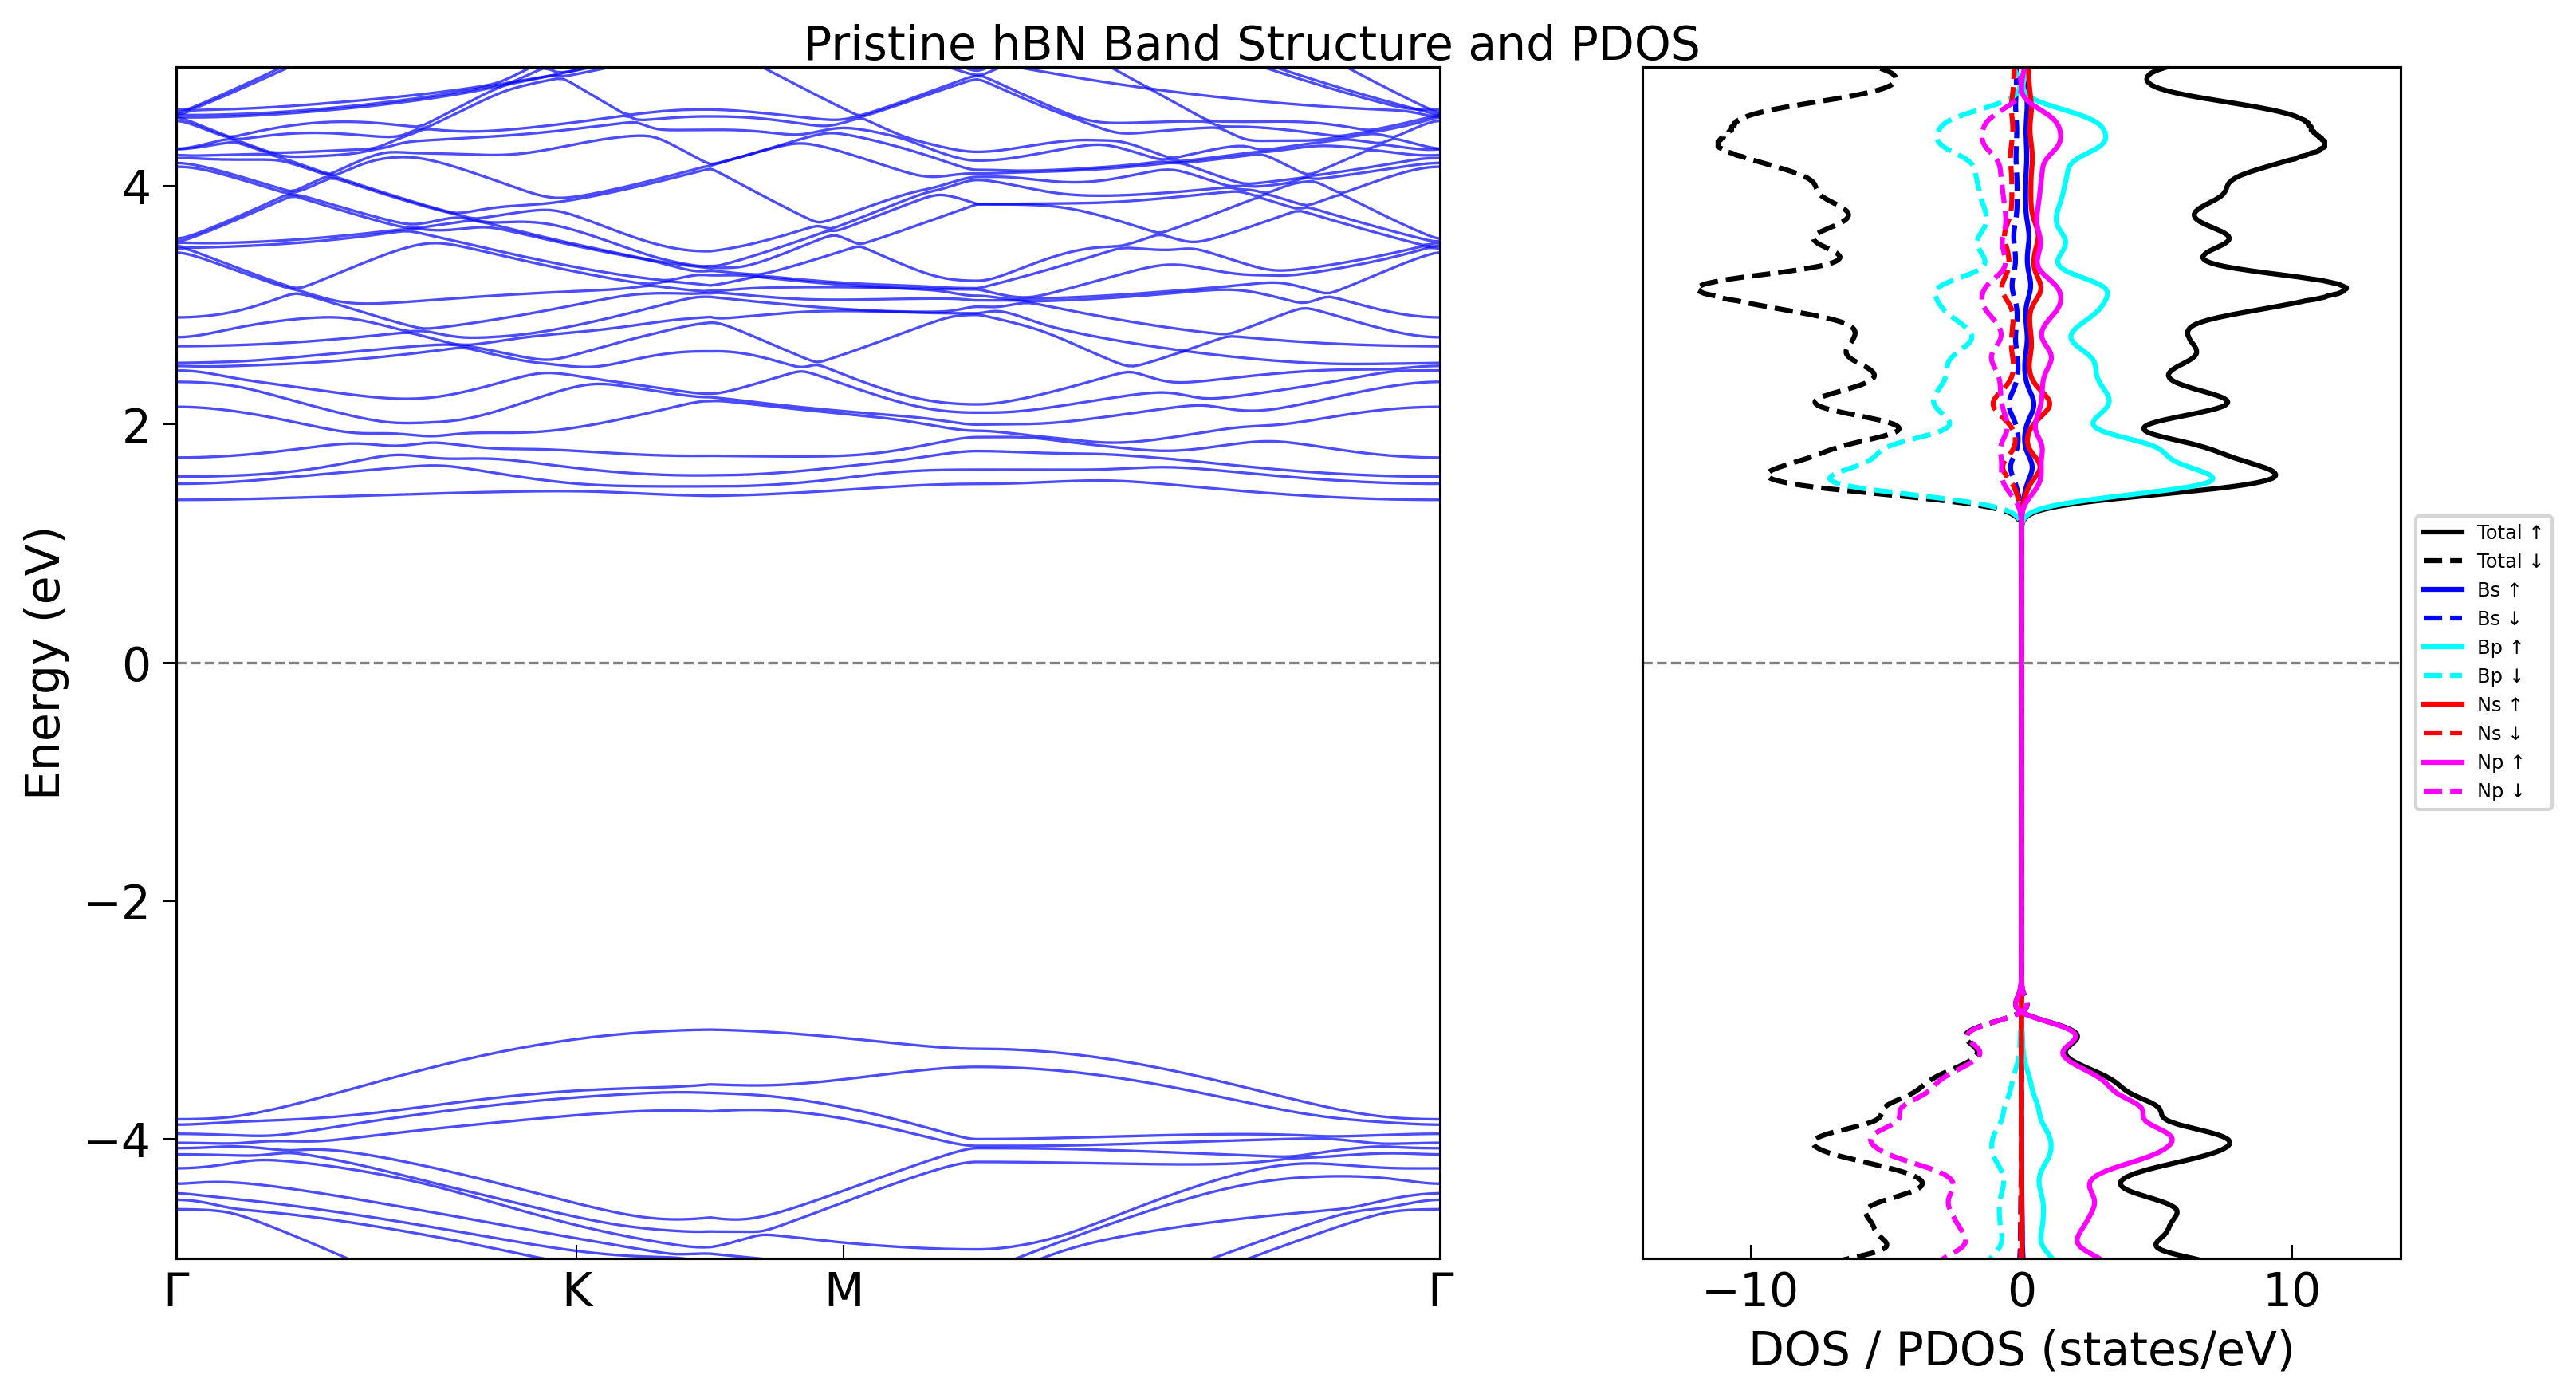
\includegraphics[width=0.9\textwidth]{gambar_hasil/simple_bands_pdos_pristine.png}
    \caption{Struktur pita elektronik dan Kerapatan Keadaan Terproyeksi (PDOS) untuk monolayer hBN murni (\textit{pristine}). Energi Fermi diset sebagai referensi energi nol pada plot PDOS.}
    \label{fig:hbn_pristine_bs_pdos}
\end{figure}

\begin{figure}[h!]
    \centering
    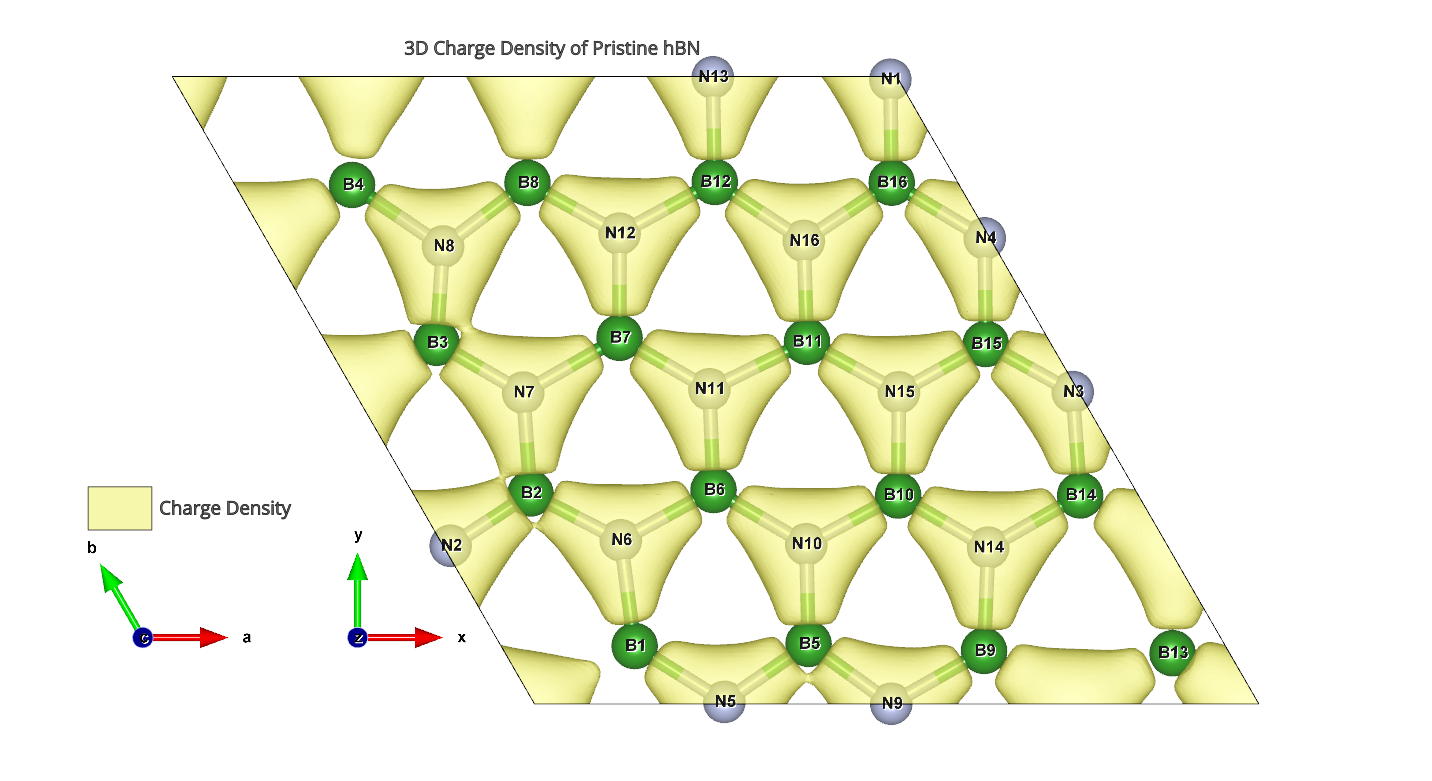
\includegraphics[width=0.9\textwidth]{gambar_hasil/hBN_rho_3d_pristine.png}
    \caption{Visualisasi kerapatan muatan elektronik 3D untuk monolayer hBN murni (\textit{pristine}). Warna menunjukkan isosurface dari kerapatan muatan.}
    \label{fig:hbn_pristine_chargedensity}
\end{figure}

\begin{figure}[h!]
    \centering
    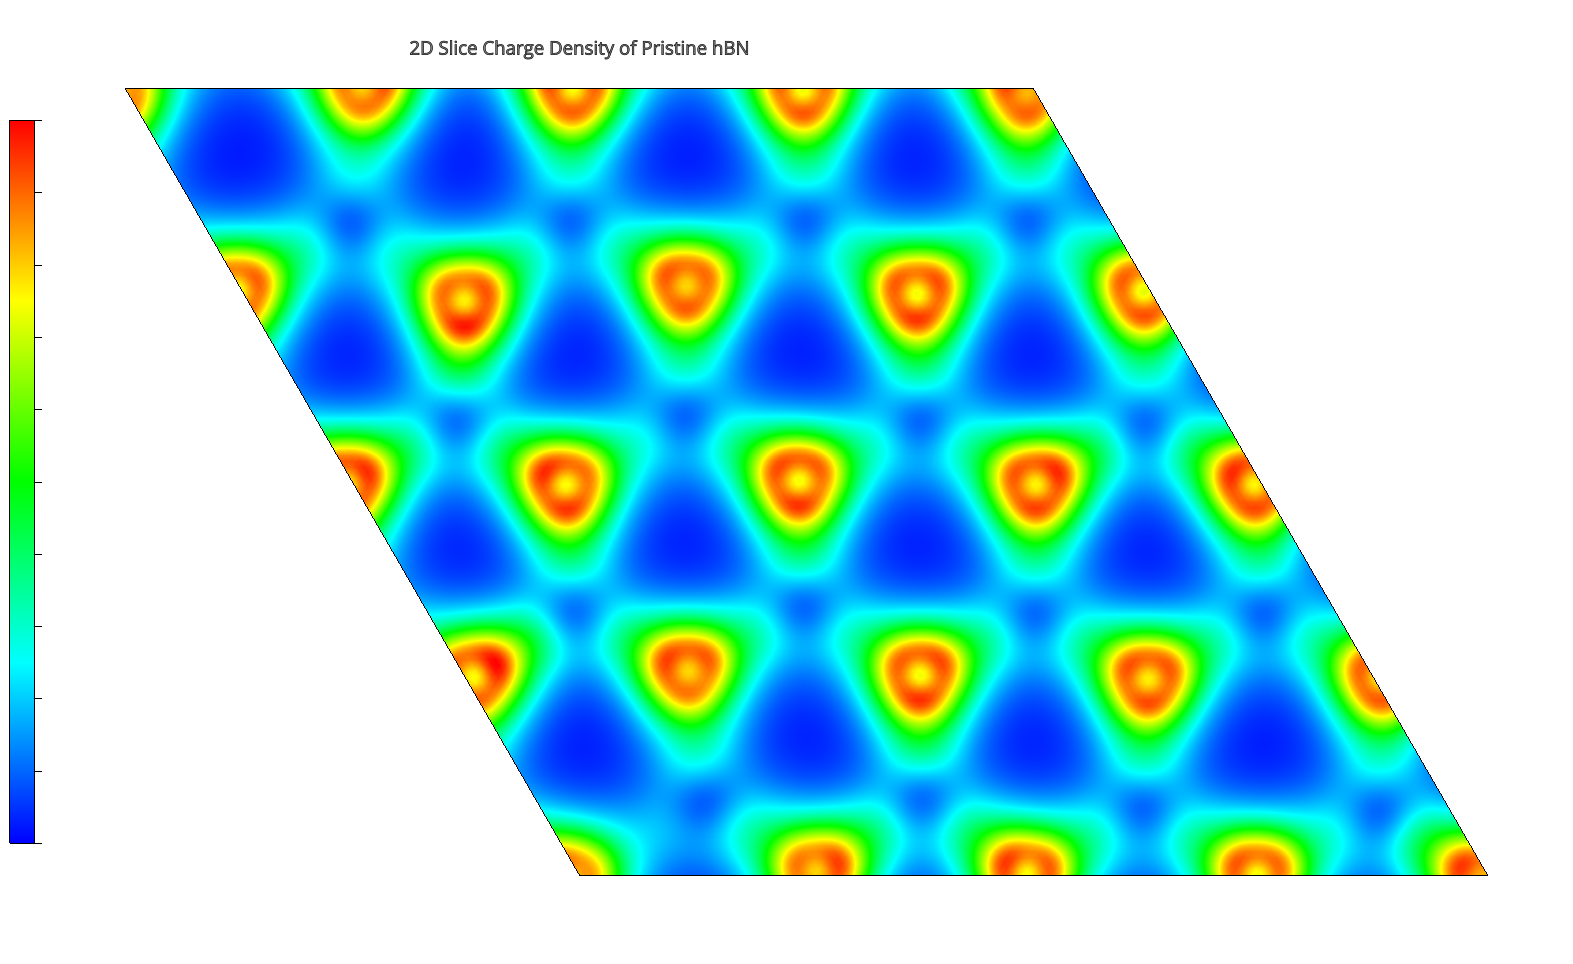
\includegraphics[width=0.9\textwidth]{gambar_hasil/hBN_rho_pristine.png}
    \caption{Visualisasi 2D dari kerapatan muatan elektronik terintegrasi-z untuk monolayer hBN murni. Warna yang lebih terang menunjukkan akumulasi muatan yang lebih tinggi di sekitar situs atom Nitrogen yang elektronegatif, menggarisbawahi sifat polar dari ikatan B-N.}
    \label{fig:hbn_pristine_chargedensity_2D}
\end{figure}

Nilai celah pita $4.446$ eV, meskipun mengalami underestimasi yang tipikal untuk fungsional GGA, konsisten dengan hasil PBE/PBEsol lain di literatur (Tabel \ref{tab:hbn_murni_literatur_updated}). Perbandingan ini memvalidasi metodologi DFT yang digunakan sebagai dasar yang reliabel untuk menganalisis perubahan relatif pada sifat elektronik.

\begin{table}[h!]
  \centering
  \caption{Perbandingan Sifat Elektronik Monolayer hBN Murni Hasil Perhitungan dengan Nilai Literatur.}
  \label{tab:hbn_murni_literatur_updated}
  \begin{threeparttable}
    \begin{tabular}{lcccc}
      \toprule
      Properti & Nilai Terhitung & Literatur & Literatur & Eksperimental \\
               & (Penelitian Ini) & PBE (eV)   & Hibrid/GW (eV) & (eV)         \\
      \midrule
      VBM (eV)  & -3.081    
      & $\sim -3.8$\tnote{a}      & $\sim -4.5$ hingga $-4.2$ & – \\
      CBM (eV)  & 1.365           & $\sim 0.8$\tnote{a}       & $\sim 1.6$ hingga $1.9$   & – \\
      $E_g$ (eV)& 4.446           & $4.66$–$4.74$             & $\sim 5.8$–$7.1$     
     & $\sim 5.9$–$6.1$ \\
      $E_F$ (eV)& -0.445          & Bervariasi\tnote{b}       & Bervariasi\tnote{b}       & Bervariasi\tnote{b} \\
      \bottomrule
    \end{tabular}
    \begin{tablenotes}[flushleft]
      \footnotesize
      \item[a] Nilai absolut VBM dan CBM sangat bergantung pada penyelarasan level vakum dan dapat bervariasi antar studi. Nilai yang ditampilkan berasal dari \citep{liu2024}.
      \item[b] Tingkat Fermi ($E_F$) berada di tengah celah pita untuk sistem murni (intrinsik), namun nilai absolutnya bergantung pada referensi energi (misalnya, level vakum).
      \item Sumber literatur: PBE/PBEsol: \citep{liu2024,korkmaz2020}; Hibrid/GW: \citep{arnaud2006}; Eksperimental: \citep{Watanabe2004}.
    \end{tablenotes}
  \end{threeparttable}
\end{table}

\subsection{Pengaruh Perlakuan Termal pada hBN Murni (800K, 1100K, dan 1225K)}
\label{subsec:hbn_murni_termal}
Untuk menginvestigasi pengaruh temperatur, struktur atomik hasil relaksasi MD pada 800K, 1100K, dan 1225K digunakan sebagai input untuk kalkulasi DFT. Hasilnya (Tabel \ref{tab:hbn_murni_suhu} dan Gambar \ref{fig:hbn_pure_800K}-\ref{fig:hbn_pure_1225K}) menunjukkan tren penurunan celah pita energi ($E_g$) seiring meningkatnya temperatur, dari $4.446$ eV (\textit{pristine}) menjadi $4.069$ eV (1225K). Penurunan total sekitar $0.377$ eV ini dikenal sebagai pergeseran merah (\textit{redshift}) termal.

\begin{table}[h!]
  \centering
  \caption{Sifat Elektronik Monolayer hBN Murni sebagai Fungsi Temperatur.}
  \label{tab:hbn_murni_suhu}
  \begin{tabular}{lccccc}
    \toprule
    Temperatur (K) & VBM (eV) & CBM (eV) & $E_g$ (eV) & $\Delta E_g$ dari Pristine (eV) & $E_F$ (eV) \\
    \midrule
    Pristine (Ref.) & -3.081 &  1.365 & 4.446 &  0.000 & -0.445 \\
    800             & -3.238 &  1.177 & 4.415 & -0.031 & -0.304 \\
    1100            & -3.183 &  1.145 & 4.328 & -0.118 & -0.323 \\
    1225            & -3.112 &  0.957 & 4.069 & -0.377 & -0.430 \\
    \bottomrule
  \end{tabular}
\end{table}

\begin{figure}[h!]
    \centering
    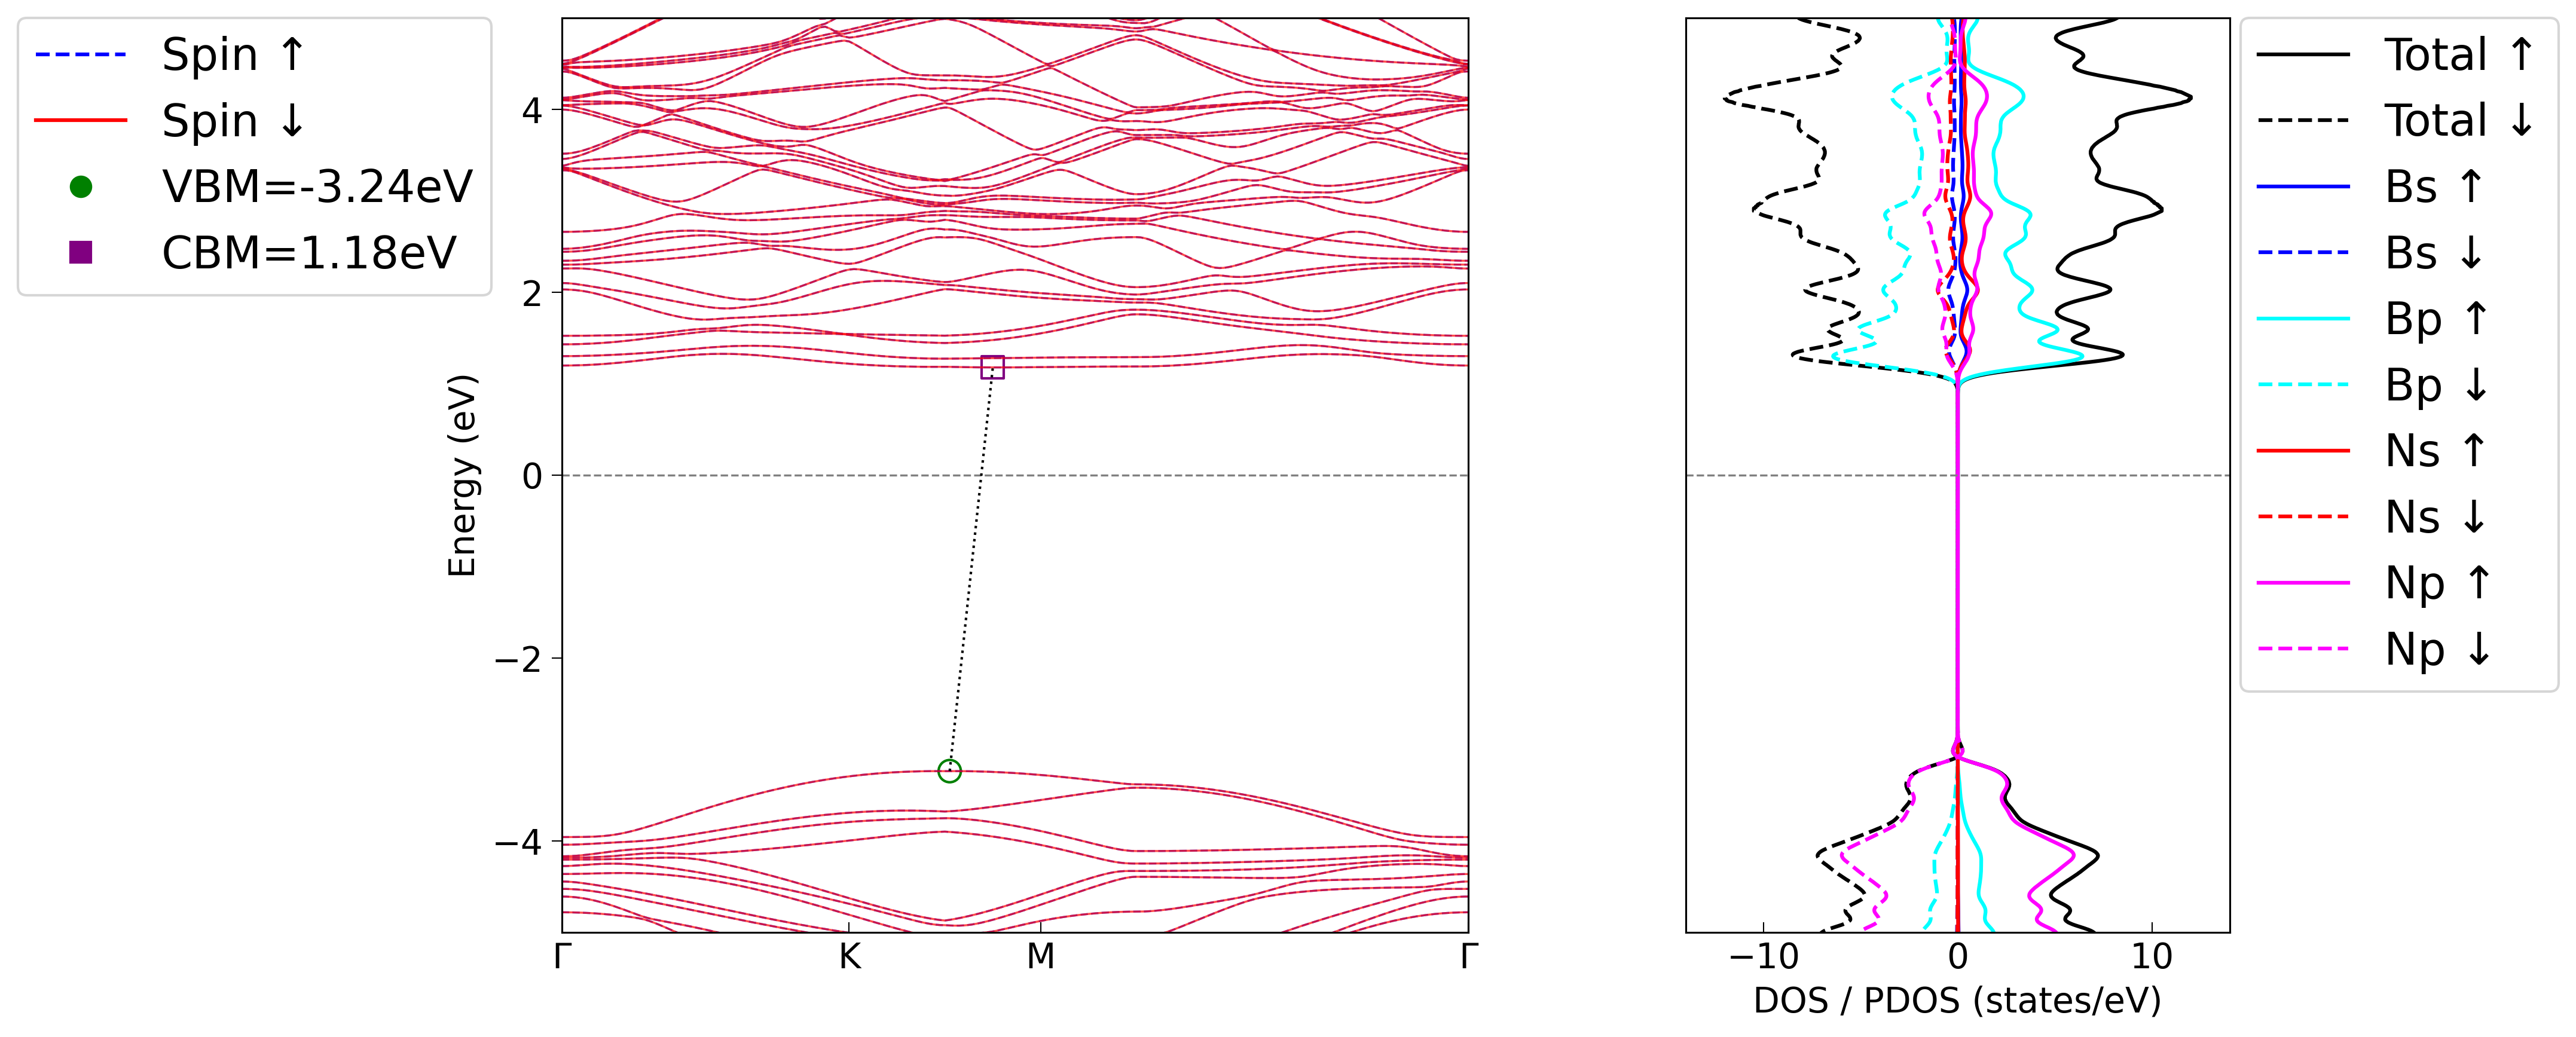
\includegraphics[width=0.9\textwidth]{gambar_hasil/simple_bands_pdos_pure_800K.png}
    \caption{Struktur pita elektronik dan PDOS untuk monolayer hBN murni pada 800K.}
    \label{fig:hbn_pure_800K}
\end{figure}

\begin{figure}[h!]
    \centering
    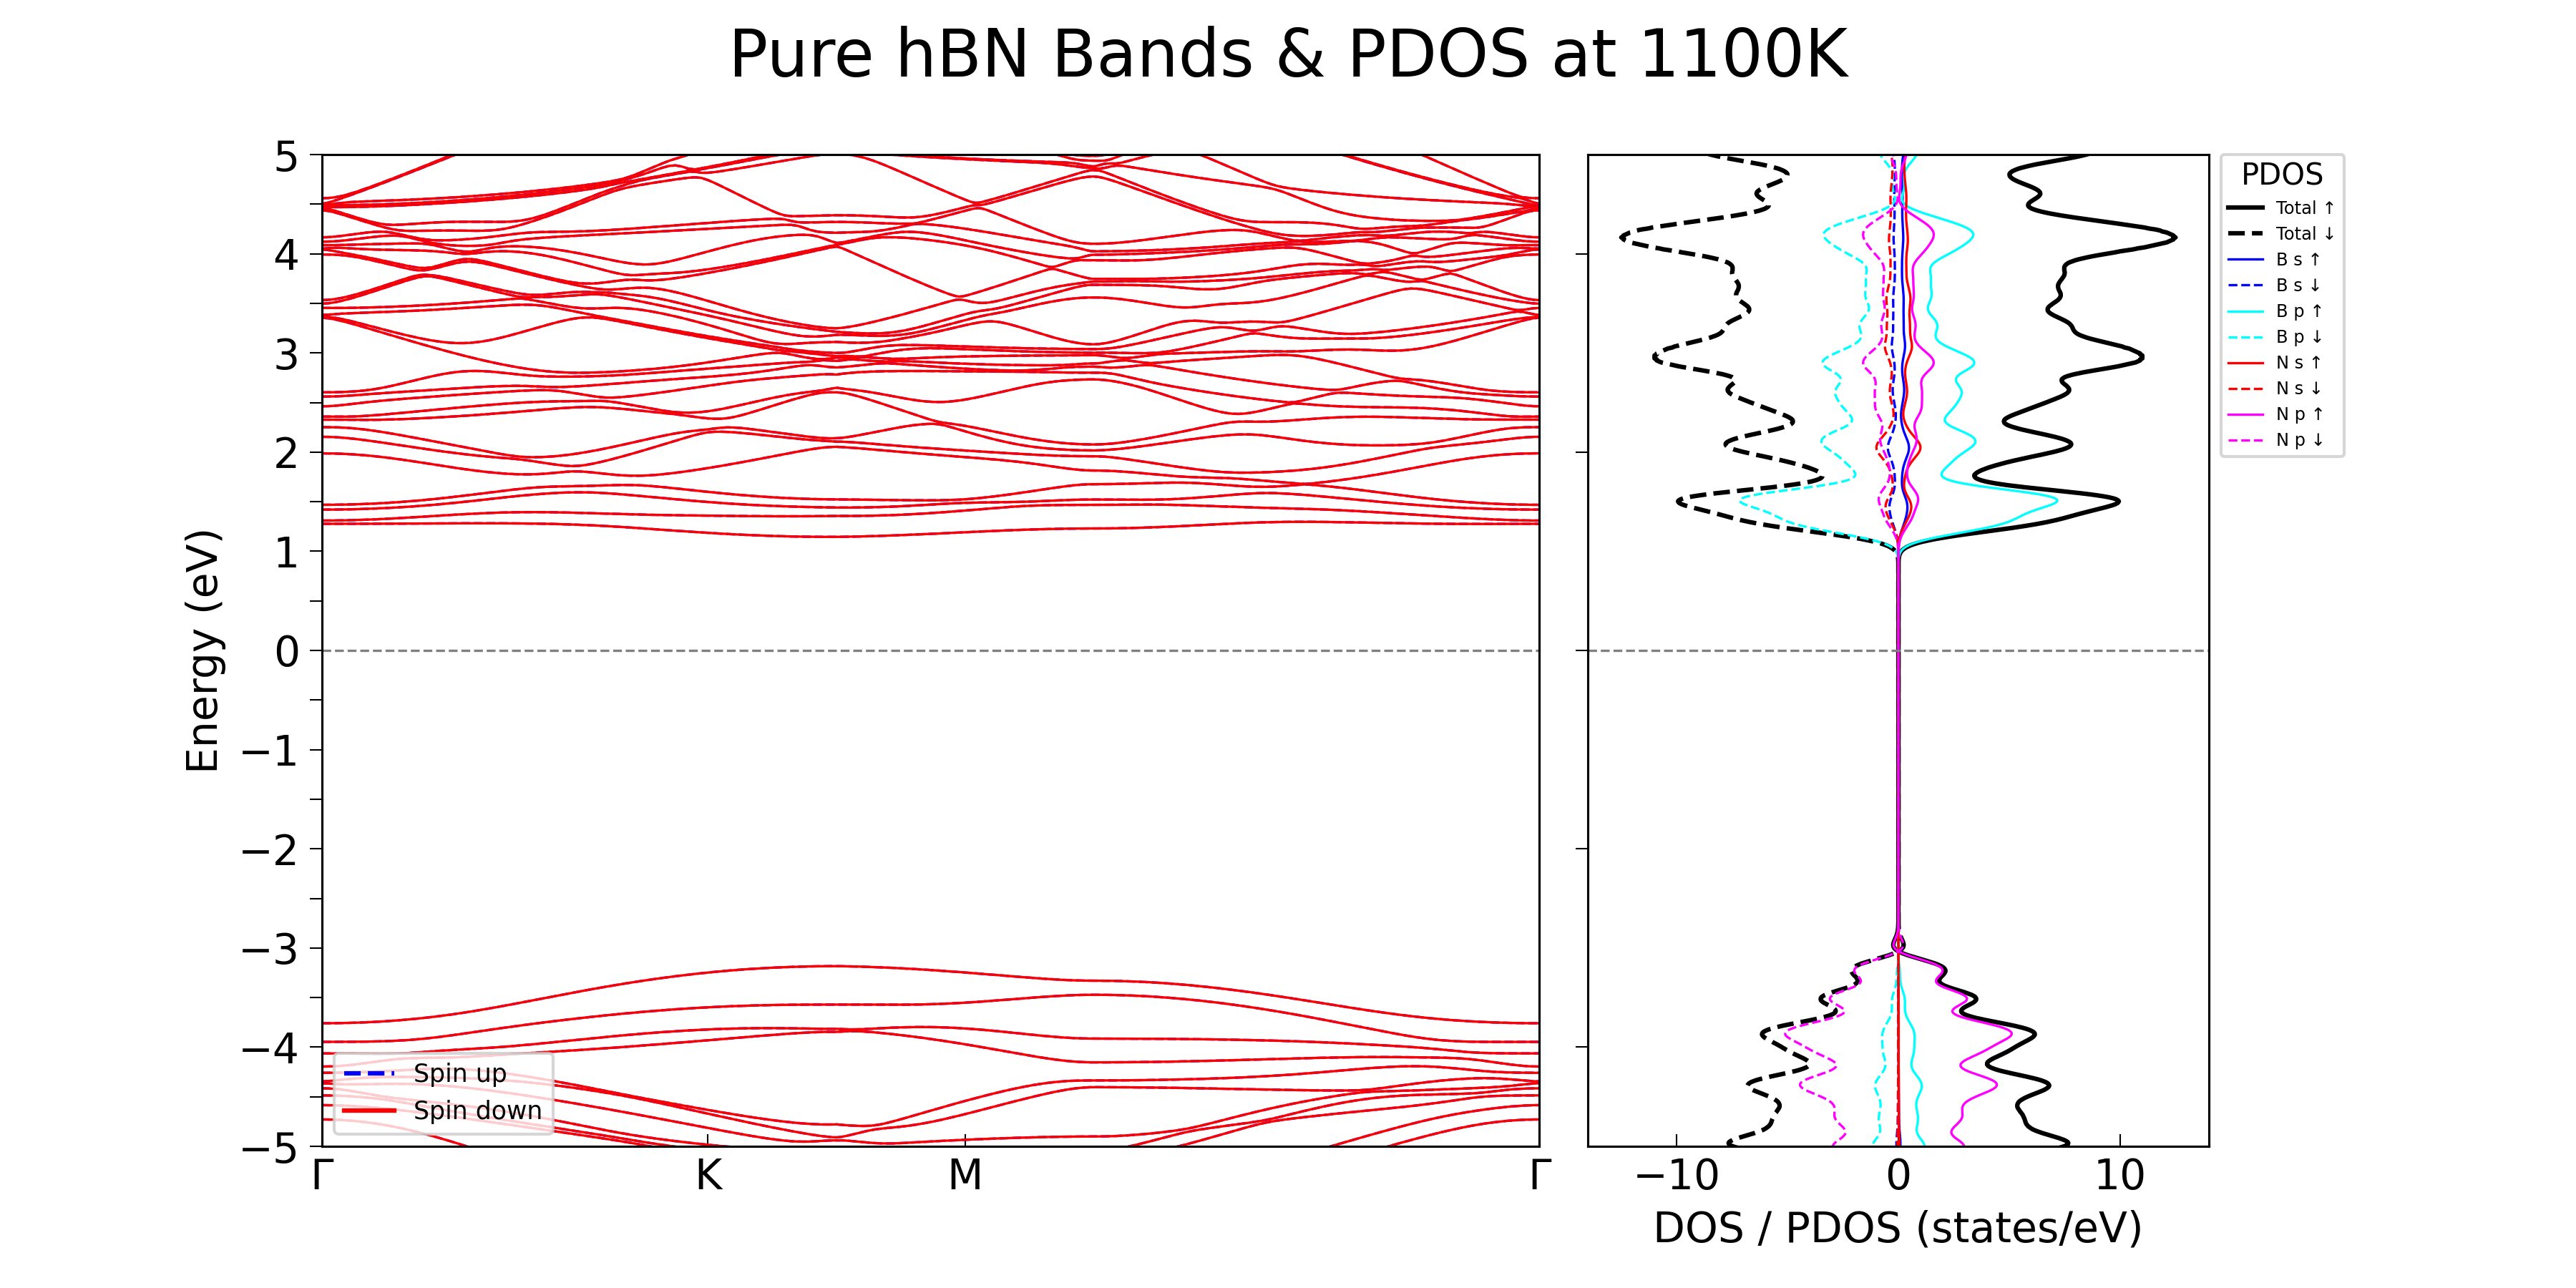
\includegraphics[width=0.9\textwidth]{gambar_hasil/simple_bands_pdos_pure_1100K.png}
    \caption{Struktur pita elektronik dan PDOS untuk monolayer hBN murni pada 1100K.}
    \label{fig:hbn_pure_1100K}
\end{figure}

\begin{figure}[h!]
    \centering
    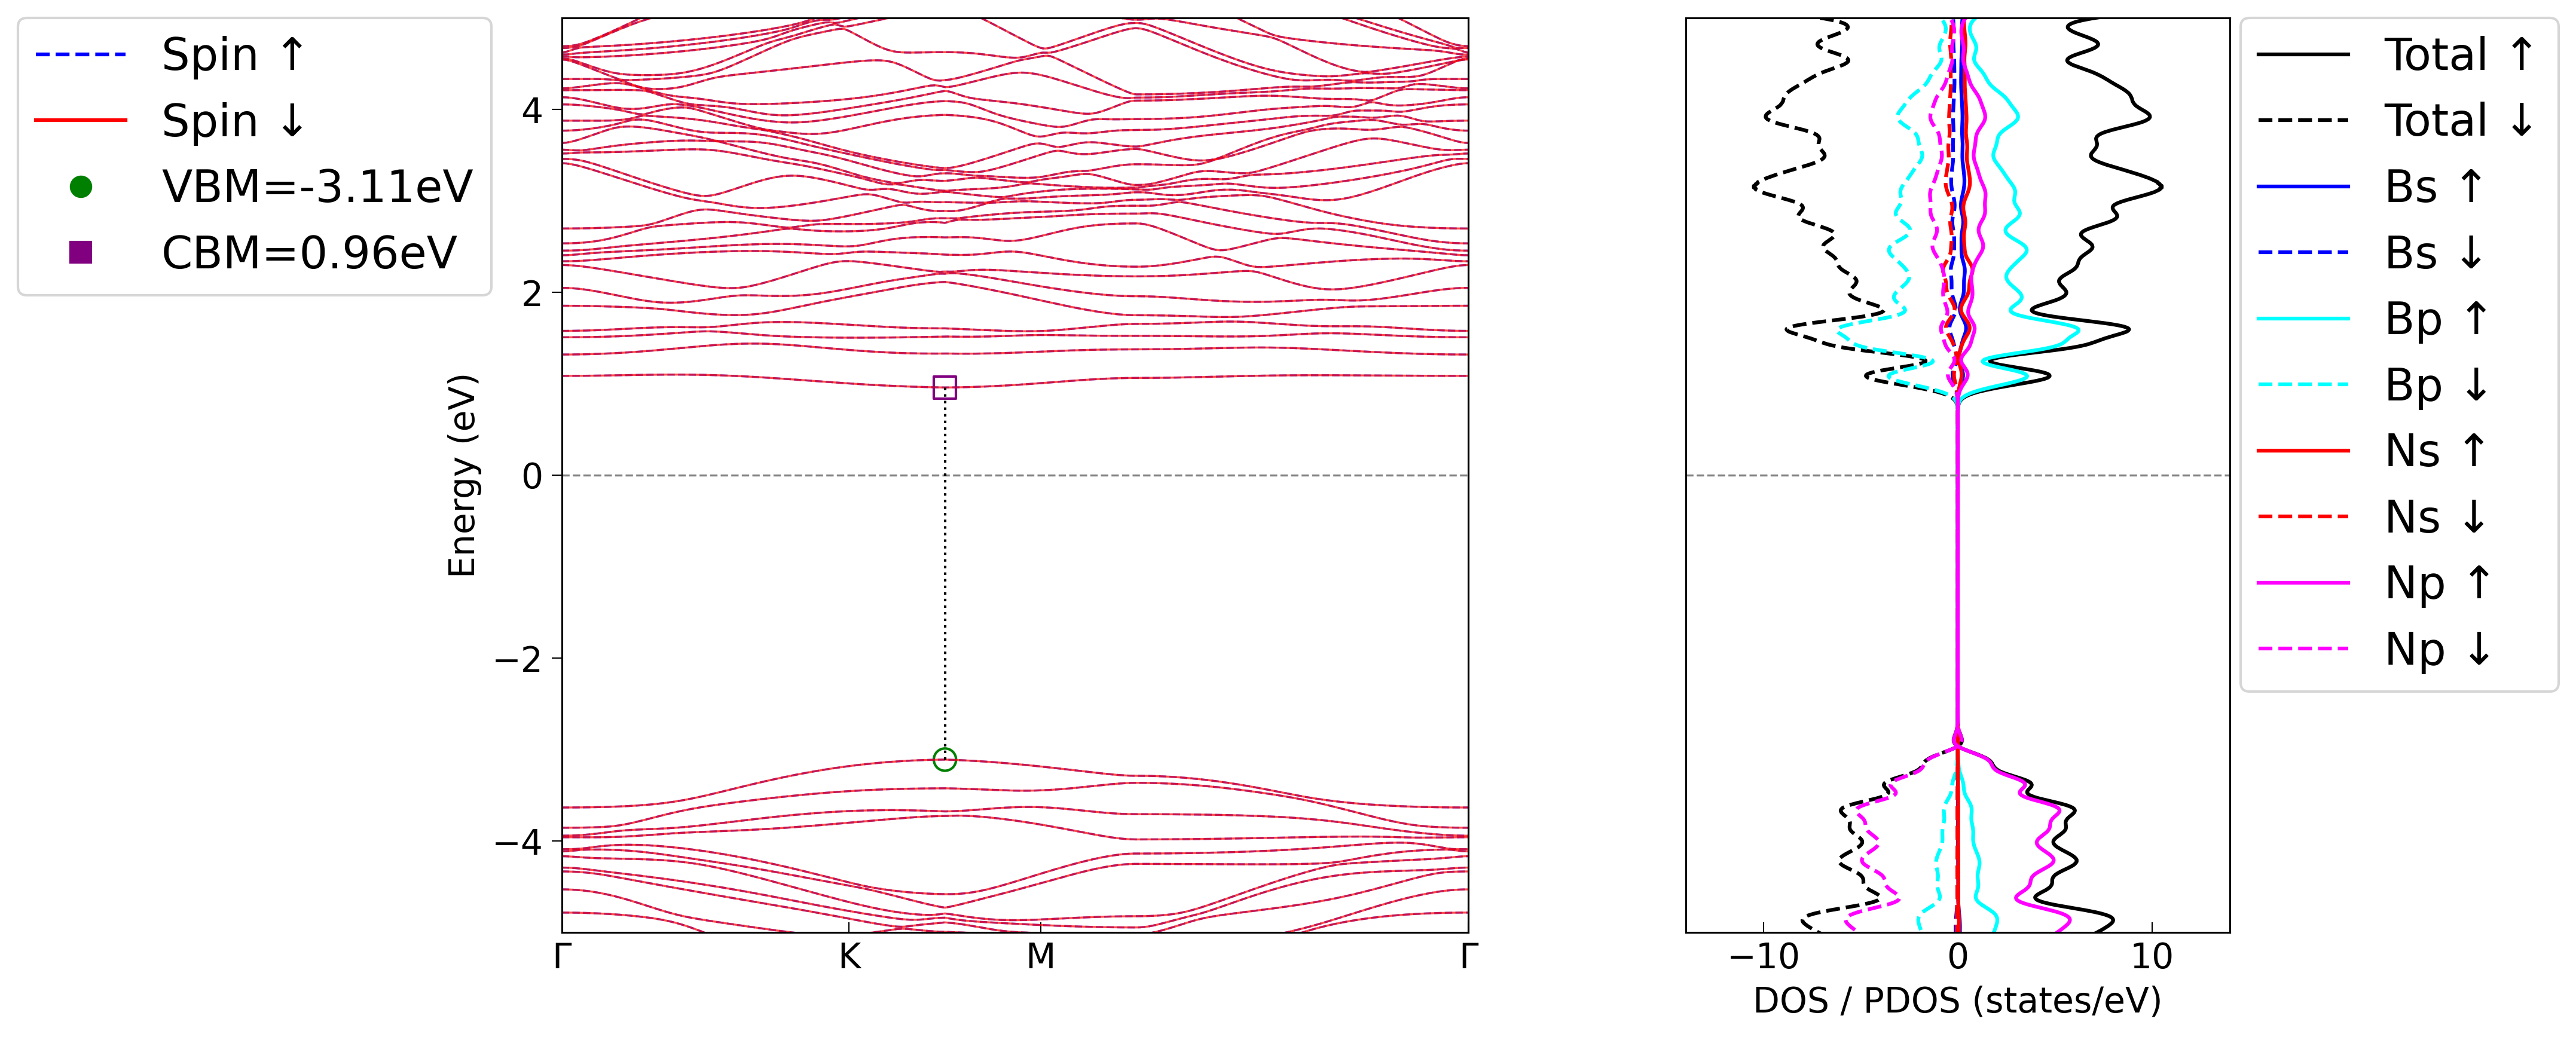
\includegraphics[width=0.9\textwidth]{gambar_hasil/simple_bands_pdos_pure_1225K.png}
    \caption{Struktur pita elektronik dan PDOS untuk monolayer hBN murni pada 1225K.}
    \label{fig:hbn_pure_1225K}
\end{figure}

Fenomena redshift termal ini merupakan ciri umum semikonduktor dan dapat dijelaskan melalui dua mekanisme utama yang terjadi secara simultan: ekspansi termal kisi dan kopling elektron-fonon (EPC).

\subsubsection{Mekanisme Kopling Elektron-Fonon dan Renormalisasi Celah Pita}
Penurunan celah pita dengan temperatur, $E_g(T)$, secara fundamental dijelaskan oleh teori interaksi elektron-fonon. Menurut kerangka teori yang dikembangkan oleh Allen, Heine, dan Cardona, perubahan $E_g$ pada volume konstan disebabkan oleh dua kontribusi utama \citep{Allen1983}.
\begin{enumerate}
    \item \textbf{Koreksi Energi-Diri Fan-Migdal:} Ini adalah kontribusi orde pertama dalam Hamiltonian interaksi elektron-fonon, yang mendeskripsikan bagaimana energi sebuah elektron direnormalisasi melalui emisi dan absorpsi virtual dari fonon. Proses ini secara efektif "membebani" elektron dengan awan fonon, yang umumnya menurunkan energinya dan juga energi CBM, sehingga mempersempit celah pita.
    \item \textbf{Kontribusi Debye-Waller (DW):} Ini adalah kontribusi orde kedua yang timbul dari fakta bahwa elektron tidak lagi bergerak dalam potensial kisi yang statis, melainkan dalam potensial yang "tercoreng" atau ter-smear akibat vibrasi termal atom. Efek ini melemahkan potensial periodik yang efektif, yang juga cenderung menurunkan energi celah pita.
\end{enumerate}
Kedua kontribusi ini, bersama dengan efek ekspansi termal (yang mengubah parameter kisi dan tumpang-tindih orbital), secara kolektif menghasilkan pergeseran merah yang diamati pada kebanyakan semikonduktor, termasuk hasil yang diperoleh untuk monolayer hBN dalam penelitian ini.

\subsubsection{Pergeseran Merah pada Monolayer vs. Pergeseran Biru Anomali pada Multilayer hBN}
Hasil redshift yang konsisten pada monolayer hBN dalam penelitian ini (800K-1225K) tampak kontras dengan perilaku yang dilaporkan untuk hBN multilayer. Studi eksperimental oleh Du et al. pada hBN multilayer menunjukkan perilaku yang lebih kompleks: redshift pada temperatur rendah (di bawah 100K) yang didominasi oleh EPC, diikuti oleh pergeseran biru (\textit{blueshift}) atau pelebaran celah pita pada temperatur yang lebih tinggi (di atas 100K hingga ~800K) \citep{Du2017}.

\begin{table}[h!]
  \centering
  \caption{Ringkasan Mekanisme Ketergantungan Temperatur Celah Pita pada hBN.}
  \label{tab:mekanisme_eg_temp}
  \begin{tabular}{p{0.3\textwidth} p{0.3\textwidth} p{0.3\textwidth}}
    \toprule
    \textbf{Mekanisme} & \textbf{Efek pada $E_g$} & \textbf{Asal Fisik} \\
    \midrule
    Kopling Elektron-Fonon (EPC) & Redshift (Penyempitan) & Interaksi Fan-Migdal \& Debye-Waller. Dominan di hampir semua semikonduktor. \\
    \addlinespace
    Ekspansi Termal Negatif (NTE) & Blueshift (Pelebaran) & Fonon lentur (flexural phonons) moda ZA yang menyebabkan kontraksi kisi dalam-bidang. \\
    \bottomrule
  \end{tabular}
\end{table}

Blueshift anomali pada hBN multilayer ini diatribusikan pada perilaku unik dari koefisien ekspansi termal negatif (\textit{Negative Thermal Expansion}, NTE) pada bidang hBN \citep{Du2017}. Mekanisme NTE pada material 2D seperti hBN dan grafena berasal dari eksitasi termal mode fonon lentur frekuensi rendah (moda ZA atau \textit{flexural phonons}) \citep{Sarikurt2022}. Vibrasi "mirip-drum" di luar bidang ini, untuk menjaga volume, secara efektif menarik atom-atom dalam bidang menjadi lebih dekat, menyebabkan kontraksi kisi saat temperatur meningkat. Kontraksi ini meningkatkan tumpang-tindih orbital dan memperlebar celah pita, bersaing dengan efek redshift dari EPC (Tabel \ref{tab:mekanisme_eg_temp}). Pada hBN multilayer, efek NTE ini menjadi dominan di atas ~100K \citep{Du2017}.

Pengamatan redshift yang konsisten pada monolayer hBN dalam penelitian ini menyoroti peran penting dimensionalitas dan, yang lebih krusial, metodologi yang digunakan. Ada beberapa kemungkinan penjelasan:
\begin{enumerate}
    \item \textbf{Dominasi EPC pada Monolayer:} Pada monolayer, tanpa adanya interaksi van der Waals antar-lapisan yang membatasi, perilaku fonon lentur mungkin berbeda. Ada kemungkinan bahwa pada rentang temperatur tinggi yang dikaji (800K-1225K), kontribusi redshift dari EPC secara inheren jauh lebih kuat daripada efek blueshift dari NTE, bahkan jika NTE terjadi.
    \item \textbf{Perbedaan Sifat Intrinsik:} Monolayer hBN memiliki celah pita langsung di titik K, sedangkan hBN multilayer memiliki celah pita tidak langsung \citep{Wickramaratne2018}. Perbedaan dalam sifat elektronik fundamental ini dapat mempengaruhi kekuatan kopling elektron-fonon di tepi pita yang relevan.
    \item \textbf{Artefak Potensial MD:} Ini adalah penjelasan yang paling kritis dan paling mungkin. Seperti yang telah dibahas di Bagian \ref{subsec:md_lammps}, potensial ReaxFF yang digunakan, yang diparameterisasi untuk sintesis fasa gas \citep{Lele2022}, kemungkinan besar tidak secara akurat menangkap anharmonicity kisi yang subtil yang bertanggung jawab atas fenomena NTE. Potensial tersebut mungkin tidak dapat mereproduksi moda fonon lentur ZA dengan benar. Akibatnya, struktur yang dihasilkan MD mungkin hanya menunjukkan ekspansi termal normal (atau tidak ada kontraksi), sehingga kalkulasi DFT berikutnya secara alami hanya akan mencerminkan efek EPC, yang selalu mengarah ke redshift.
\end{enumerate}
Dengan demikian, redshift yang teramati pada monolayer hBN harus diinterpretasikan dengan hati-hati. Fenomena ini kemungkinan besar bukan representasi lengkap dari fisika yang sebenarnya, melainkan cerminan dari fisika yang "diizinkan" oleh keterbatasan potensial interatomik yang digunakan dalam tahap MD.

\section{Dampak Defek Antisite pada Sifat Elektronik dan Magnetik hBN}
\label{sec:hbn_defek}
Kehadiran defek titik dapat secara dramatis mengubah sifat elektronik dan magnetik material. Bagian ini membahas pengaruh dua jenis defek antisite, N$_B$ (Nitrogen pada situs Boron) dan B$_N$ (Boron pada situs Nitrogen), terhadap sifat-sifat monolayer hBN. Berdasarkan data hasil kalkulasi, "NN defect" diinterpretasikan sebagai defek N$_B$, dan "BB defect" sebagai defek B$_N$.

\subsection{Monolayer hBN dengan Defek Antisite N$_B$ ("NN defect")}
\label{subsec:hbn_defek_nb}
Defek antisite N$_B$ mengintroduksi perubahan signifikan pada struktur elektronik. Hasil kalkulasi dirangkum dalam Tabel \ref{tab:hbn_defek_nb} dan diilustrasikan pada Gambar \ref{fig:hbn_NN_800K} hingga \ref{fig:hbn_NB_1225K_2D_plots}.

\begin{table}[h!]
  \centering
  \caption{Sifat Elektronik Monolayer hBN dengan Defek Antisite N$_B$ sebagai Fungsi Temperatur.}
  \label{tab:hbn_defek_nb}
  \begin{tabular}{lcccccc}
    \toprule
    Temperatur & VBM & CBM & $E_g$ & $E_F$ & Magnetisasi & Magnetisasi \\
    (K) & (eV) & (eV) & (eV) & (eV) & Total ($\mu_B$) & Absolut ($\mu_B$) \\
    \midrule
    800  & -0.448 &  0.246 & 0.694 & -2.538 & 0.000 & 0.000 \\
    1100 & -0.666 &  0.423 & 1.089 & -2.682 & 0.000 & 0.000 \\
    1225 & -0.732 &  0.482 & 1.214 & -2.237 & 0.000 & 0.010 \\
    \bottomrule
  \end{tabular}
\end{table}

\begin{figure}[h!]
    \centering
    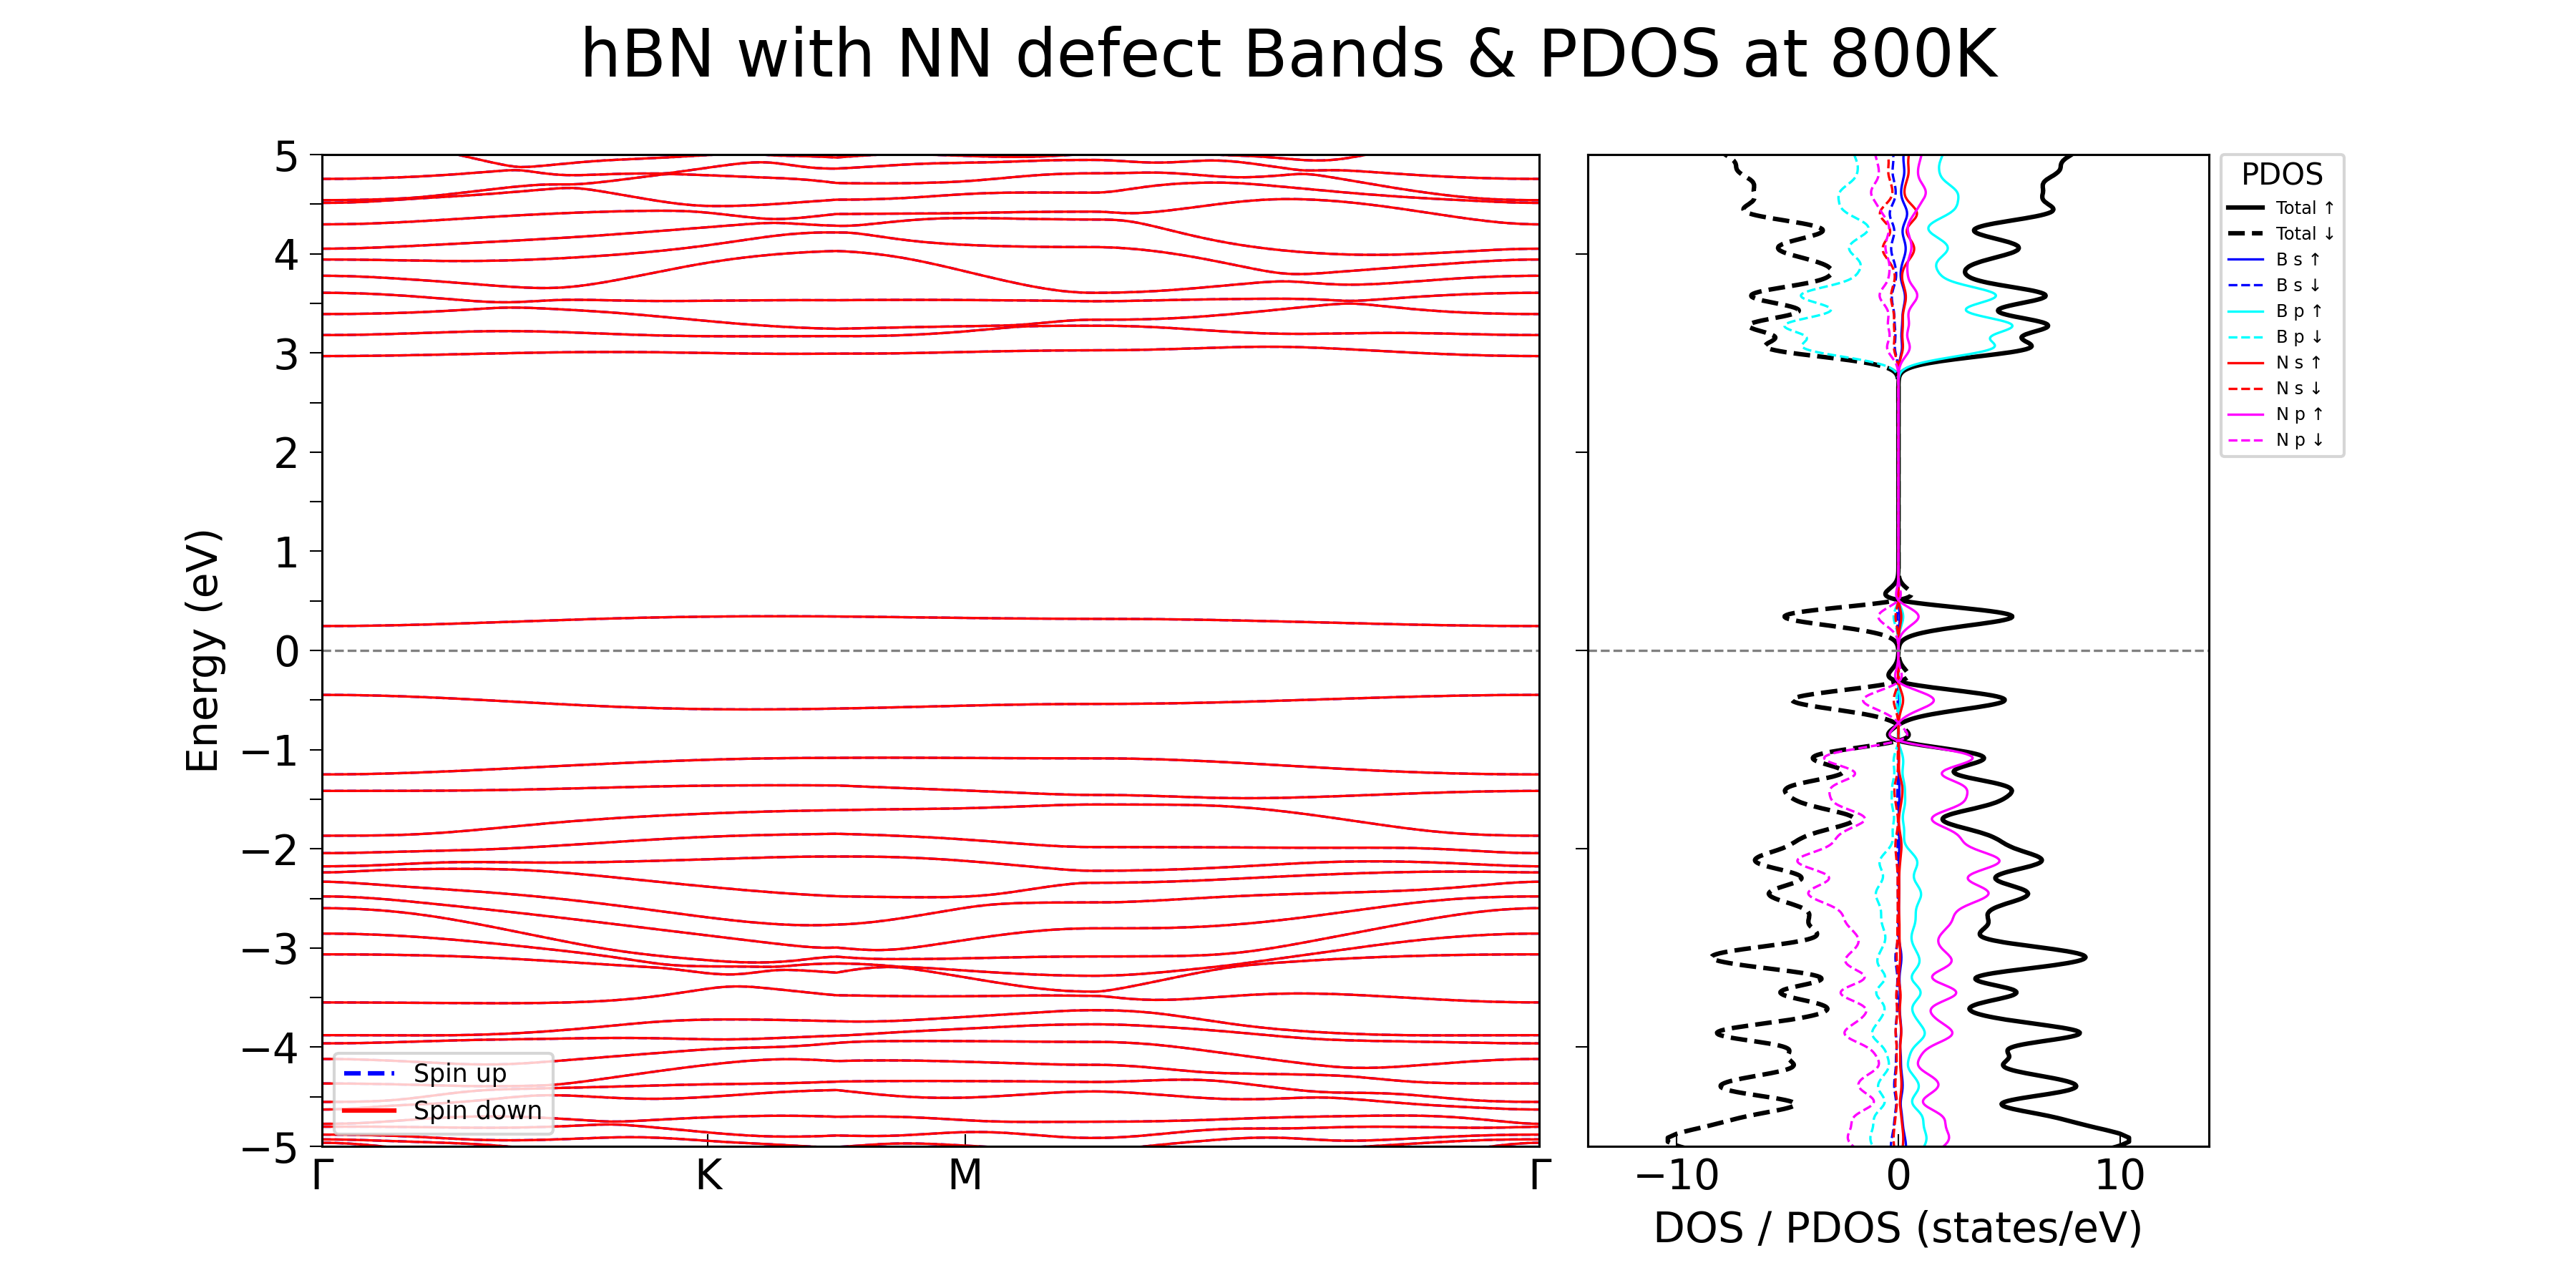
\includegraphics[width=0.9\textwidth]{gambar_hasil/simple_bands_pdos_NN_800K.png}
    \caption{Struktur pita elektronik dan PDOS untuk monolayer hBN dengan defek N$_B$ pada 800K.}
    \label{fig:hbn_NN_800K}
\end{figure}
\begin{figure}[h!]
    \centering
    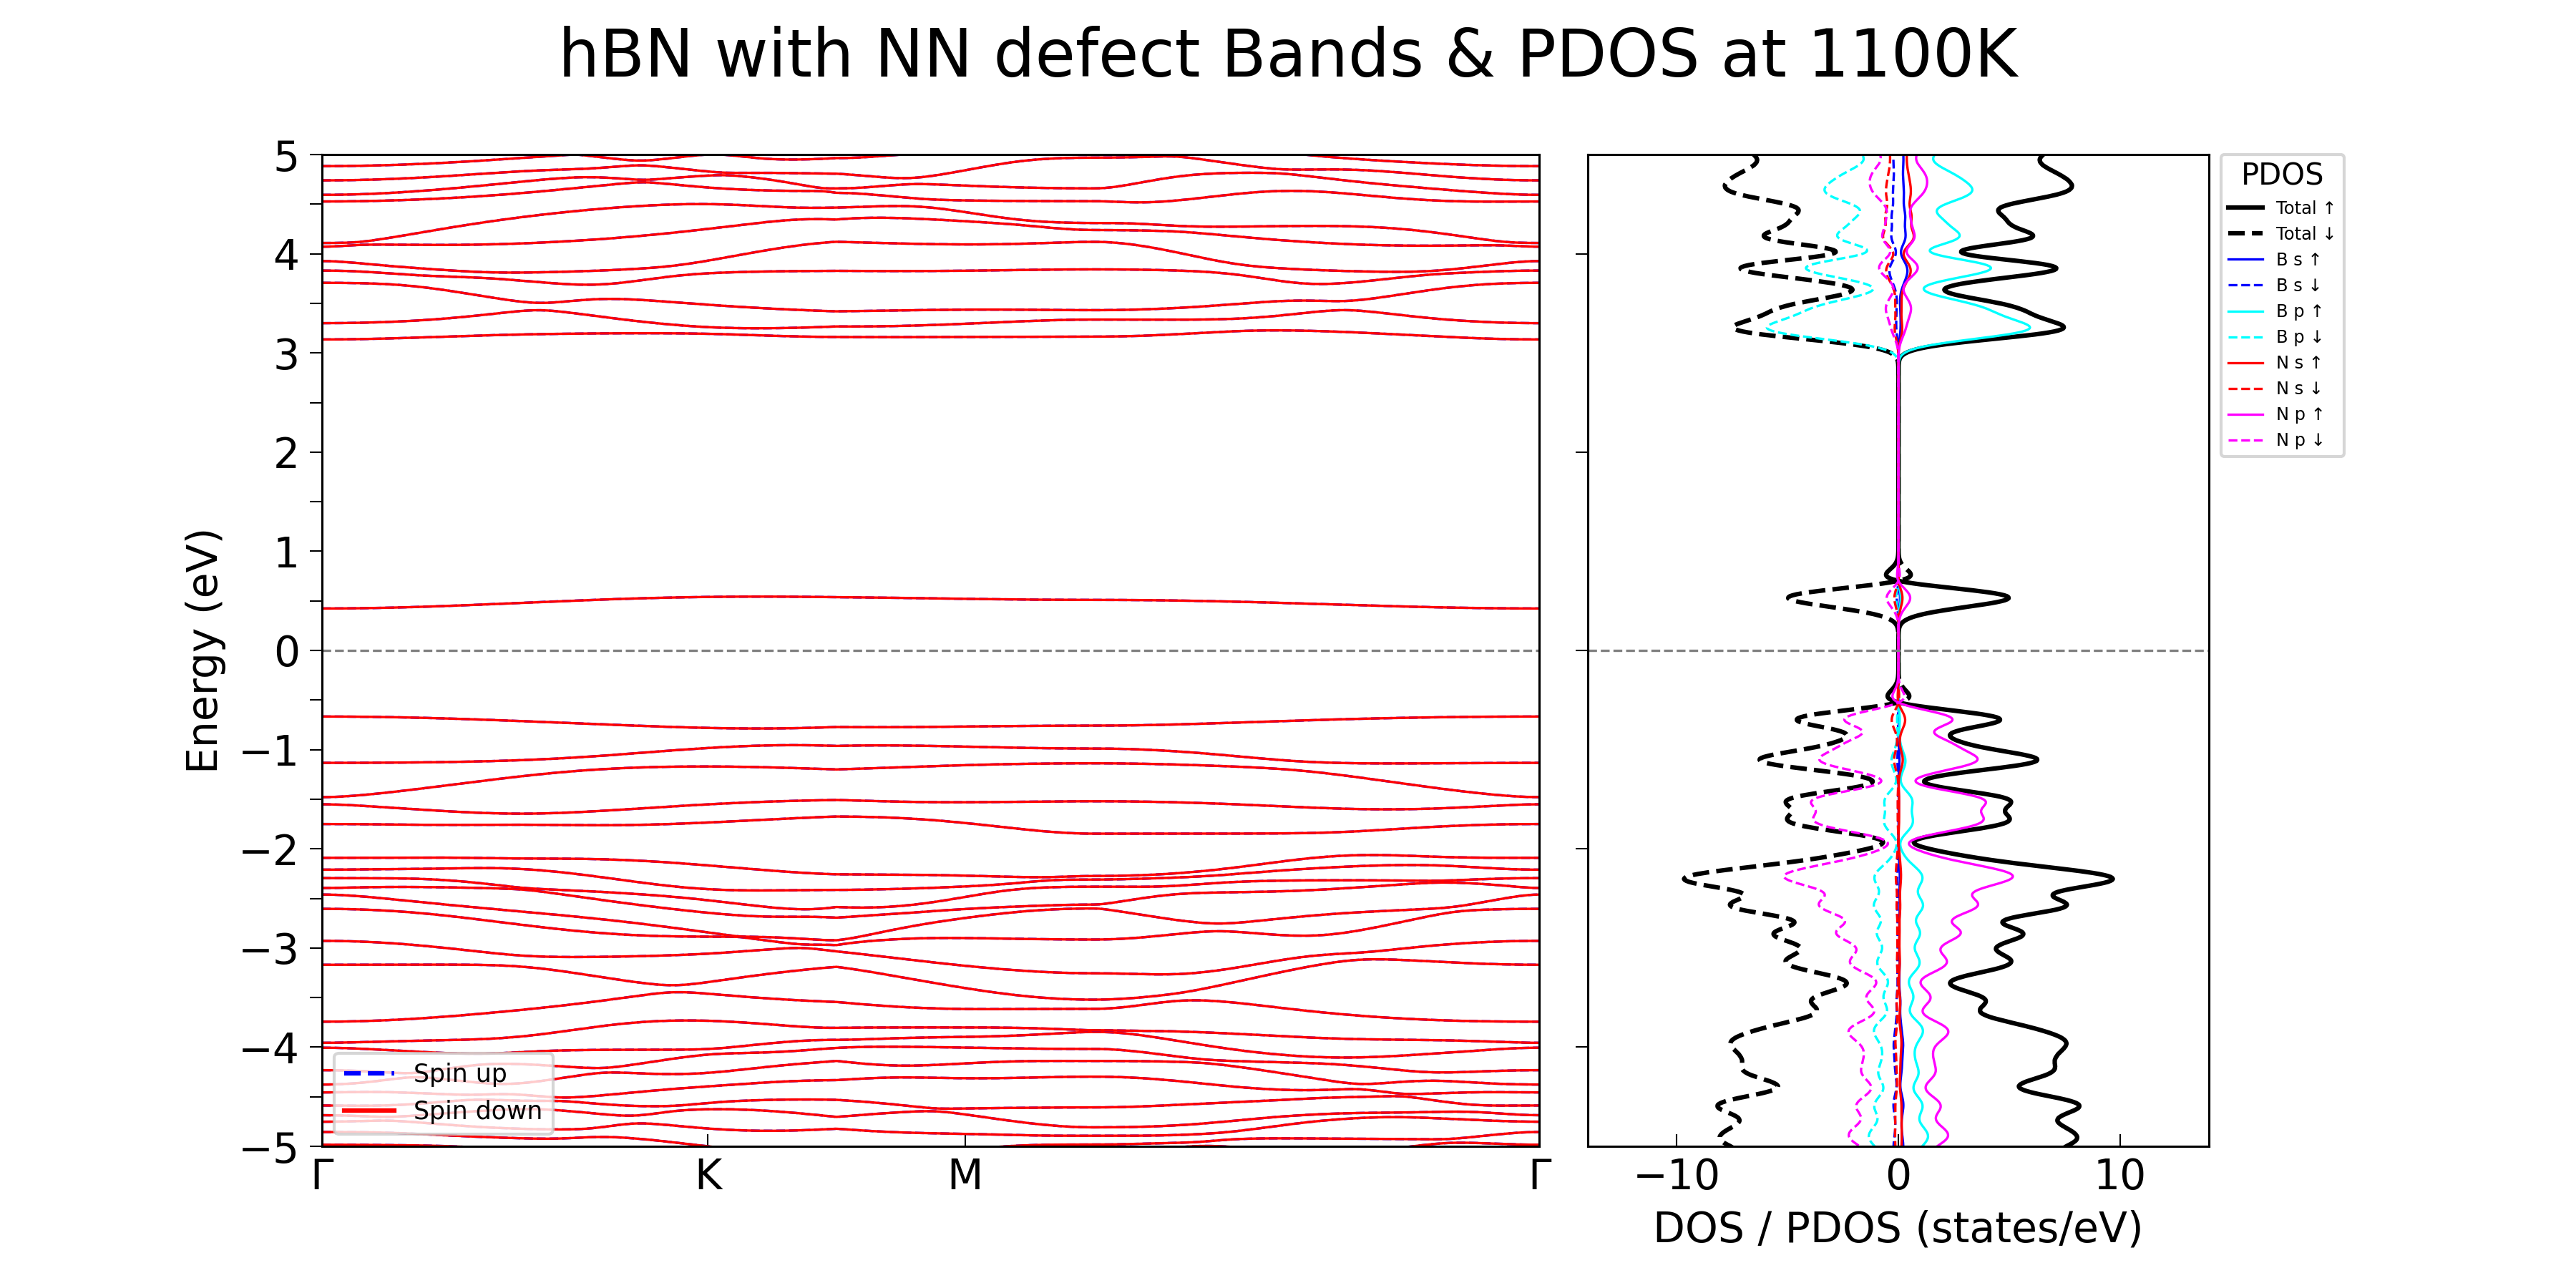
\includegraphics[width=0.9\textwidth]{gambar_hasil/simple_bands_pdos_NN_1100K.png}
    \caption{Struktur pita elektronik dan PDOS untuk monolayer hBN dengan defek N$_B$ pada 1100K.}
    \label{fig:hbn_NN_1100K}
\end{figure}
\begin{figure}[h!]
    \centering
    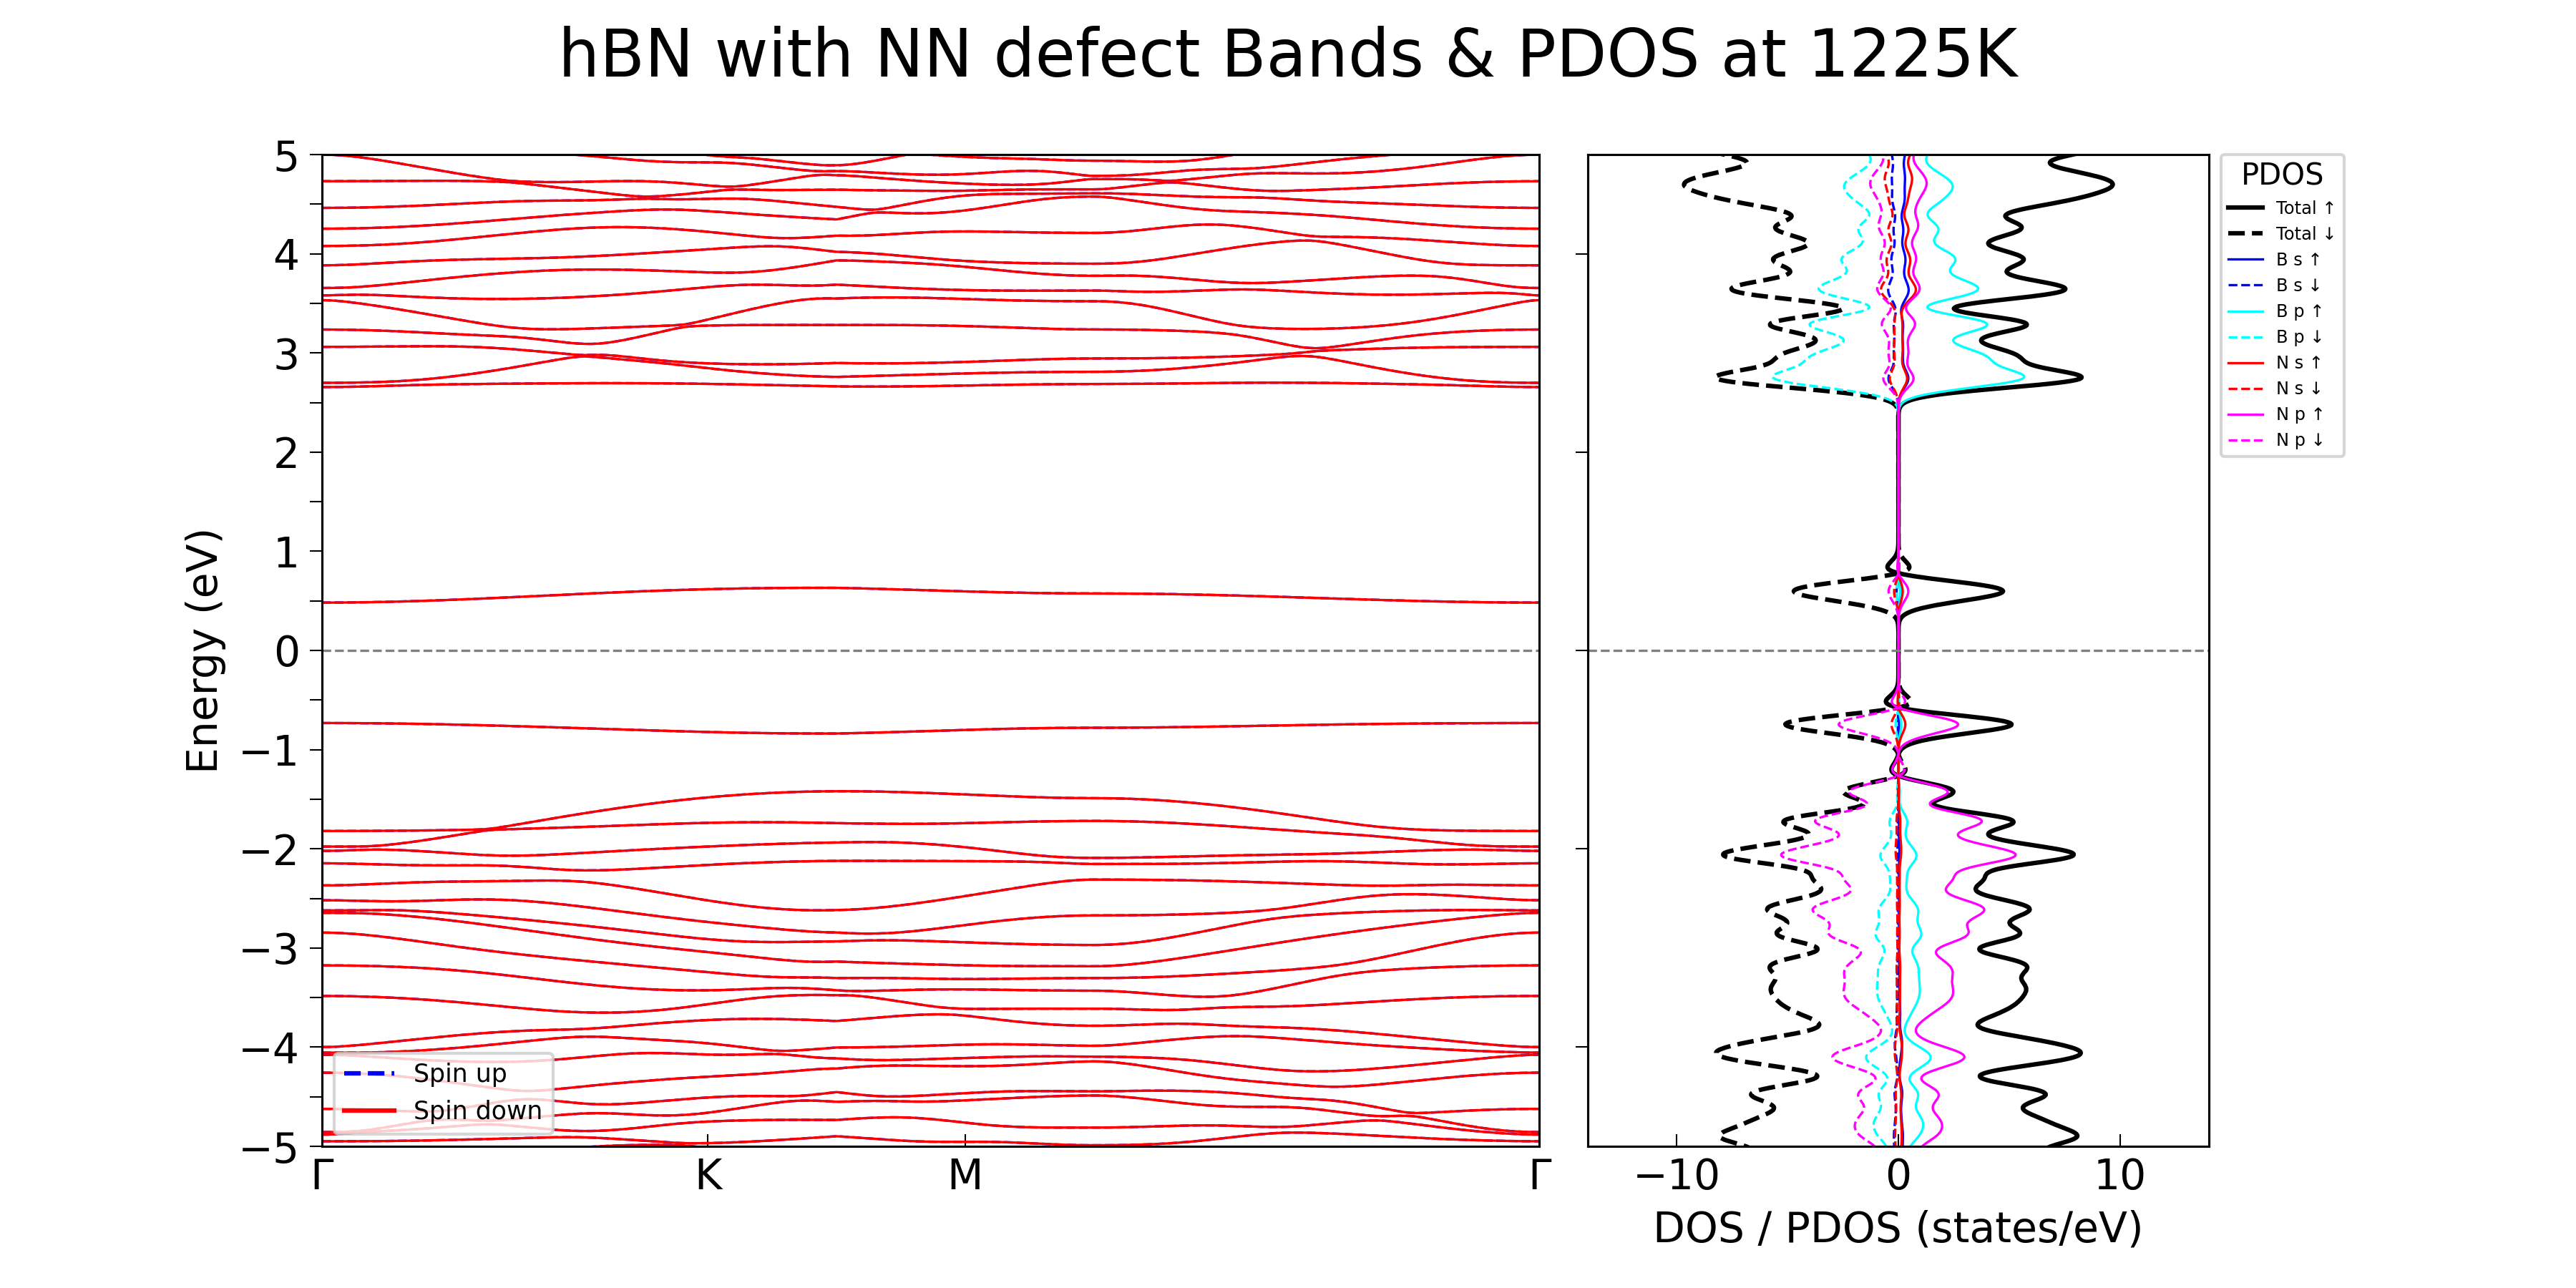
\includegraphics[width=0.9\textwidth]{gambar_hasil/simple_bands_pdos_NN_1225K.png}
    \caption{Struktur pita elektronik dan PDOS untuk monolayer hBN dengan defek N$_B$ pada 1225K.}
    \label{fig:hbn_NN_1225K}
\end{figure}
\begin{figure}[h!]
    \centering
    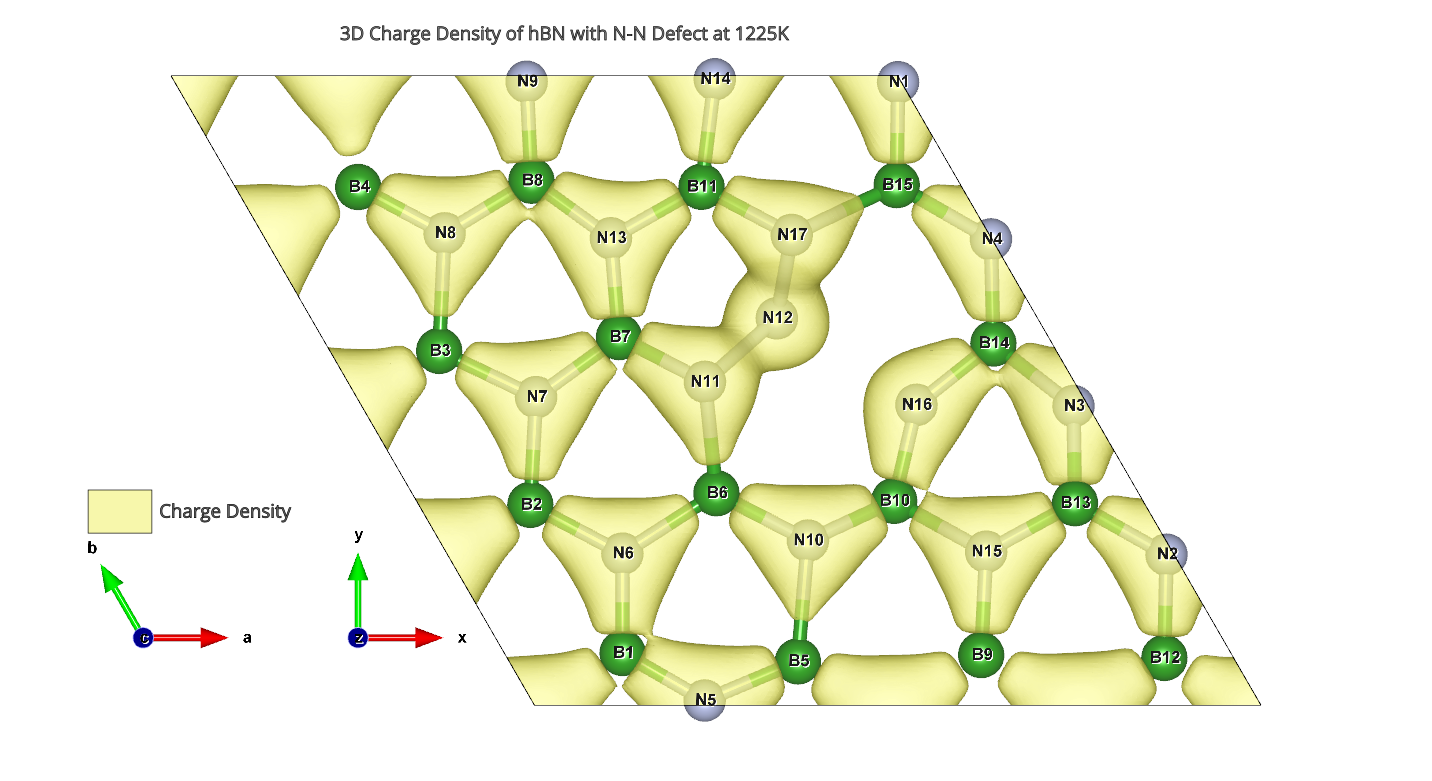
\includegraphics[width=0.6\textwidth]{gambar_hasil/hBN_rho_3D_NN_1225K.png}
    \caption{Visualisasi kerapatan muatan elektronik 3D untuk monolayer hBN dengan defek N$_B$ pada 1225K.}
    \label{fig:hbn_NN_1225K_chargedensity}
\end{figure}

\begin{figure}[h!]
    \centering
    % Subfigure pertama
    \begin{subfigure}[b]{0.45\textwidth}
        \centering
        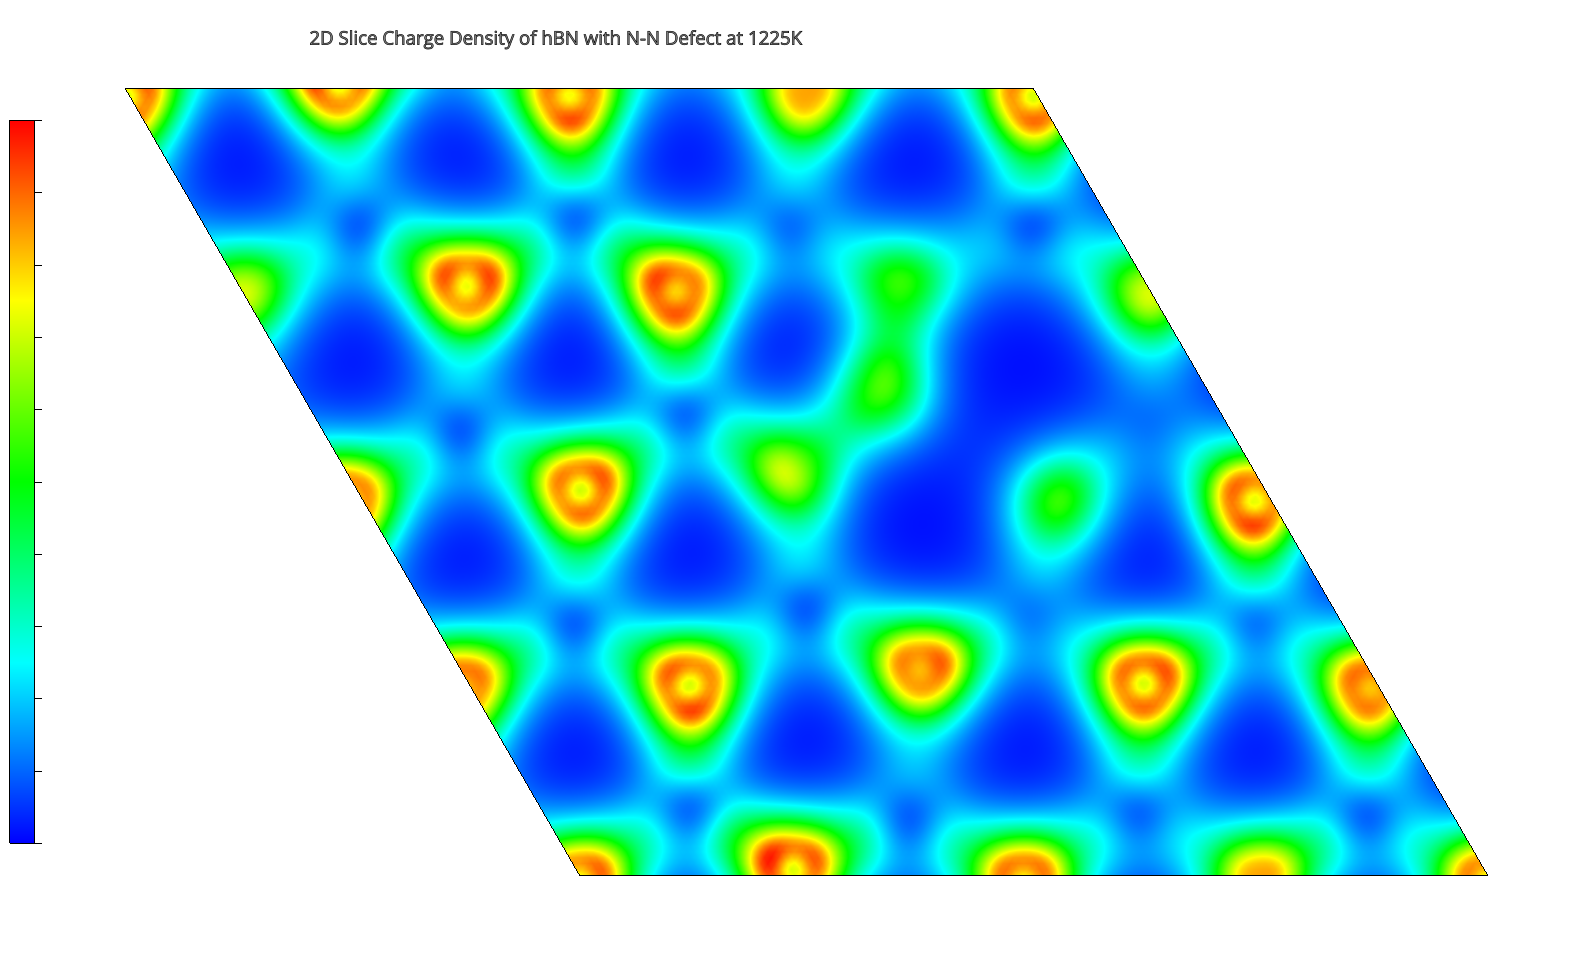
\includegraphics[width=\linewidth,height=7cm,keepaspectratio]{gambar_hasil/hBN_rho_NN_1225K.png}
        \caption{Kerapatan Muatan 2D\\Defek N$_B$ pada 1225K}
        \label{fig:2D_charge_density_NN_1225K}
    \end{subfigure}
    \hfill
    % Subfigure kedua
    \begin{subfigure}[b]{0.45\textwidth}
        \centering
        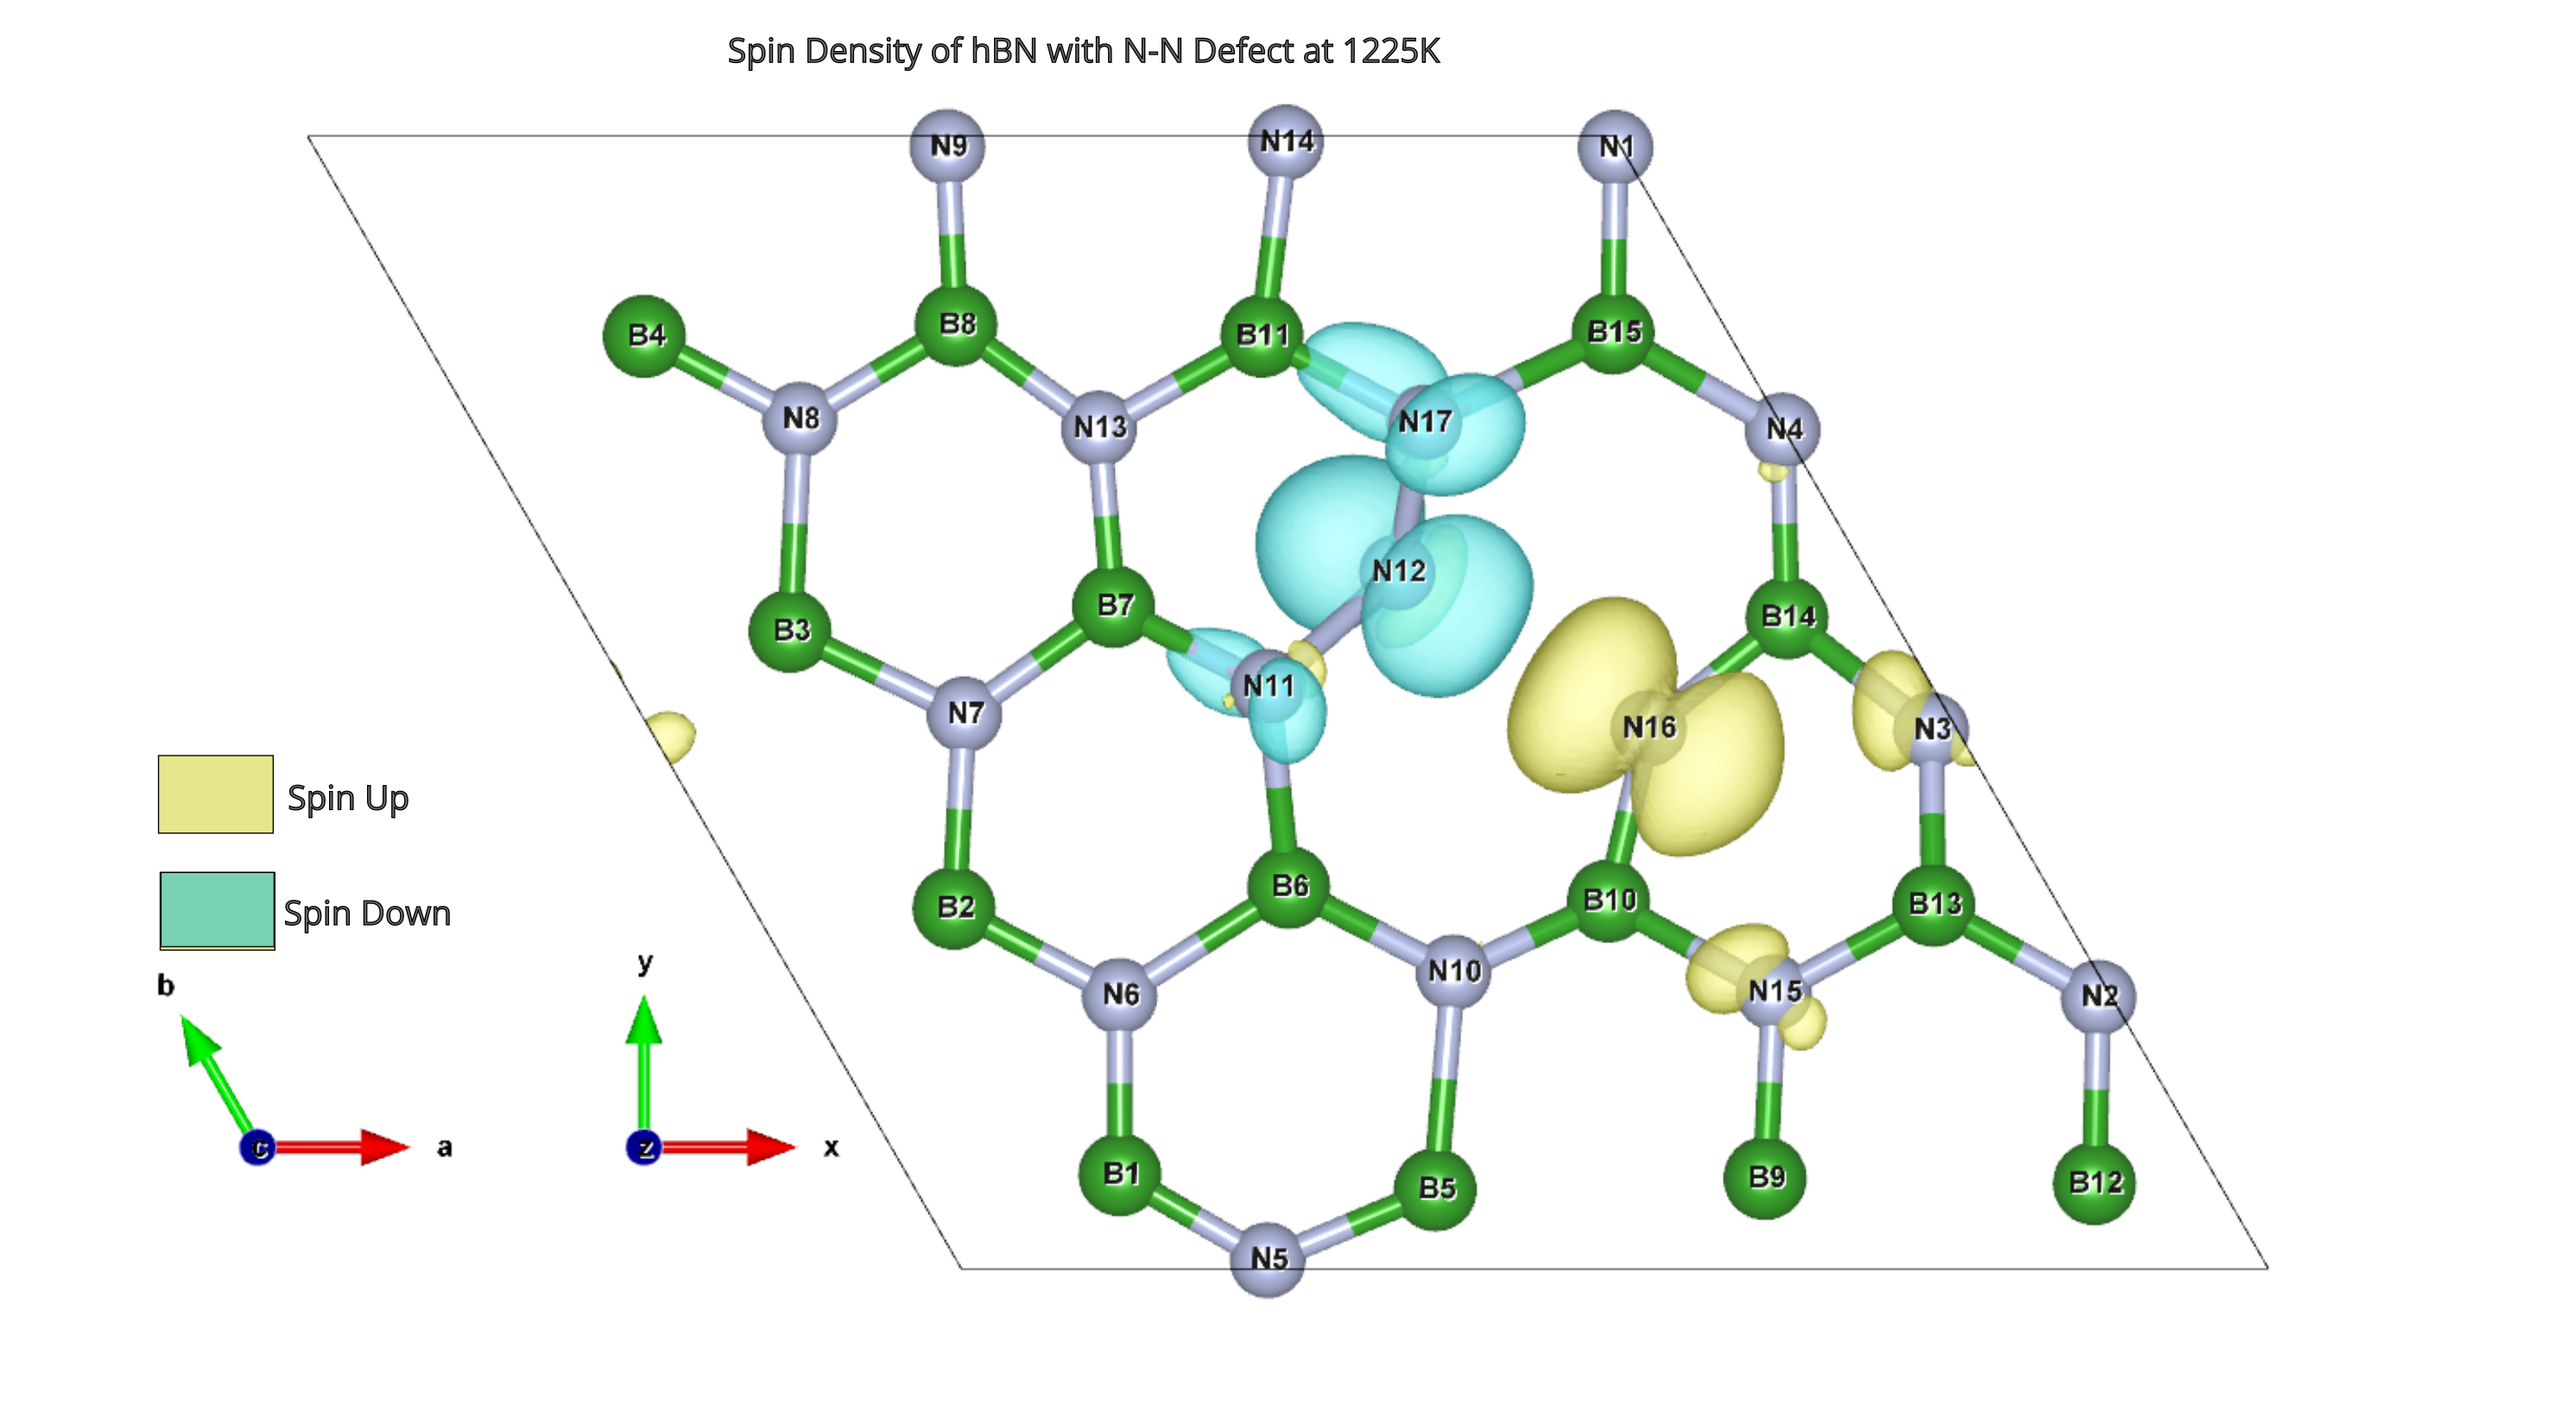
\includegraphics[width=\linewidth,height=7cm,keepaspectratio]{gambar_hasil/hBN_spin_NN_1225K.png}
        \caption{Kerapatan Spin 2D\\Defek N$_B$ pada 1225K}
        \label{fig:spin_density_NN_1225K}
    \end{subfigure}

    \caption{Visualisasi 2D untuk monolayer hBN dengan defek N$_B$ pada 1225K. 
    (a) Kerapatan muatan menunjukkan redistribusi elektron di sekitar situs defek. 
    (b) Kerapatan spin, yang diharapkan mendekati nol, mengonfirmasi sifat non-magnetik sistem ini.}
    \label{fig:hbn_NB_1225K_2D_plots}
\end{figure}

Kehadiran defek N$_B$ menyebabkan reduksi celah pita energi yang drastis (misalnya, $0.694$ eV pada 800K) akibat pembentukan tingkat-tingkat energi defek yang terlokalisasi di dalam celah pita intrinsik hBN. Tren yang paling menarik adalah ketergantungan $E_g$ terhadap temperatur: celah pita justru meningkat dengan kenaikan temperatur (blueshift), dari $0.694$ eV pada 800K menjadi $1.214$ eV pada 1225K. Perilaku anomali ini, yang berlawanan dengan tren pada hBN murni, menyiratkan bahwa keadaan-keadaan defek yang mendefinisikan VBM dan CBM efektif sangat sensitif terhadap distorsi struktural lokal di sekitar defek. Kenaikan temperatur, melalui vibrasi kisi, mengubah konfigurasi atomik lokal ini sedemikian rupa sehingga pemisahan energi antara keadaan defek terisi dan tak terisi menjadi lebih besar. Ini adalah manifestasi dari kopling elektron-fonon yang kuat dan terlokalisasi pada situs defek \citep{Grosso2020,ozan2025}.

Sistem tetap non-magnetik pada semua temperatur (momen magnetik absolut 0.010 $\mu_B$ pada 1225K kemungkinan besar adalah noise numerik). Namun, perilaku elektronik yang sangat tidak biasa ini, ditambah dengan label "NN defect" dari file kalkulasi, menimbulkan pertanyaan apakah ini benar-benar defek N$_B$ tunggal yang sederhana. Literatur terbaru menunjukkan bahwa defek kaya-Nitrogen yang lebih kompleks, seperti \textit{nitrogen split interstitial} (dimer N-N pada satu situs kisi), bisa jadi merupakan kandidat yang lebih mungkin untuk beberapa emitor di hBN \citep{ganyecz2024}. Defek semacam ini, yang secara efektif memiliki ikatan N-N, akan memiliki struktur elektronik dan respons termal yang sangat berbeda dari N$_B$ tunggal dan bisa menjelaskan perilaku anomali yang teramati. Ada kemungkinan bahwa selama simulasi MD pada suhu tinggi, dinamika atomik yang kompleks mengarah pada pembentukan struktur defek yang lebih rumit daripada antisite tunggal yang dimaksudkan.


\subsection{Monolayer hBN dengan Defek Antisite B$_N$ ("BB defect")}
\label{subsec:hbn_defek_bn}
Defek antisite Boron (B$_N$) menginduksi perubahan yang lebih dramatis, terutama pada sifat magnetiknya. Data hasil kalkulasi dirangkum dalam Tabel \ref{tab:hbn_defek_bn} dan diilustrasikan pada Gambar \ref{fig:hbn_BB_800K} hingga \ref{fig:hbn_BB_1225K_2D_plots}.

\begin{table}[h!]
  \centering
  \caption{Sifat Elektronik dan Magnetik Monolayer hBN dengan Defek Antisite B$_N$ sebagai Fungsi Temperatur.}
  \label{tab:hbn_defek_bn}
  \resizebox{\textwidth}{!}{%
  \begin{tabular}{lcccccccccc}
    \toprule
    Temperatur & VBM & CBM & $E_g$ Sistem & $E_F$ & Mag. Total & Mag. Abs. & Momen Orbital & Momen Orbital & Momen Orbital & Momen Orbital \\
    (K) & (eV) & (eV) & Total (eV) & (eV) & ($\mu_B$) & ($\mu_B$) & B-s ($\mu_B$) & B-p ($\mu_B$) & N-s ($\mu_B$) & N-p ($\mu_B$) \\
    \midrule
    800  & -0.633 & 0.357 & 0.990 & -0.249 & 0.000 & 0.000 & -0.000 & 0.000 & -0.000 & 0.000 \\
    1100 & -0.120 ($\downarrow$) & 0.301 ($\uparrow$)  & 0.421 & -0.410 & 0.150 & 0.230 &  0.003 & 0.010 & -0.000 & 0.001 \\
    1225 & -0.073 ($\uparrow$) & 0.243 ($\downarrow$)  & 0.316 & -0.622 & 1.850 & 2.320 &  0.057 & 0.009 & -0.022 & -0.002 \\
    \bottomrule
  \end{tabular}%
  }
\end{table}

\begin{figure}[h!]
    \centering
    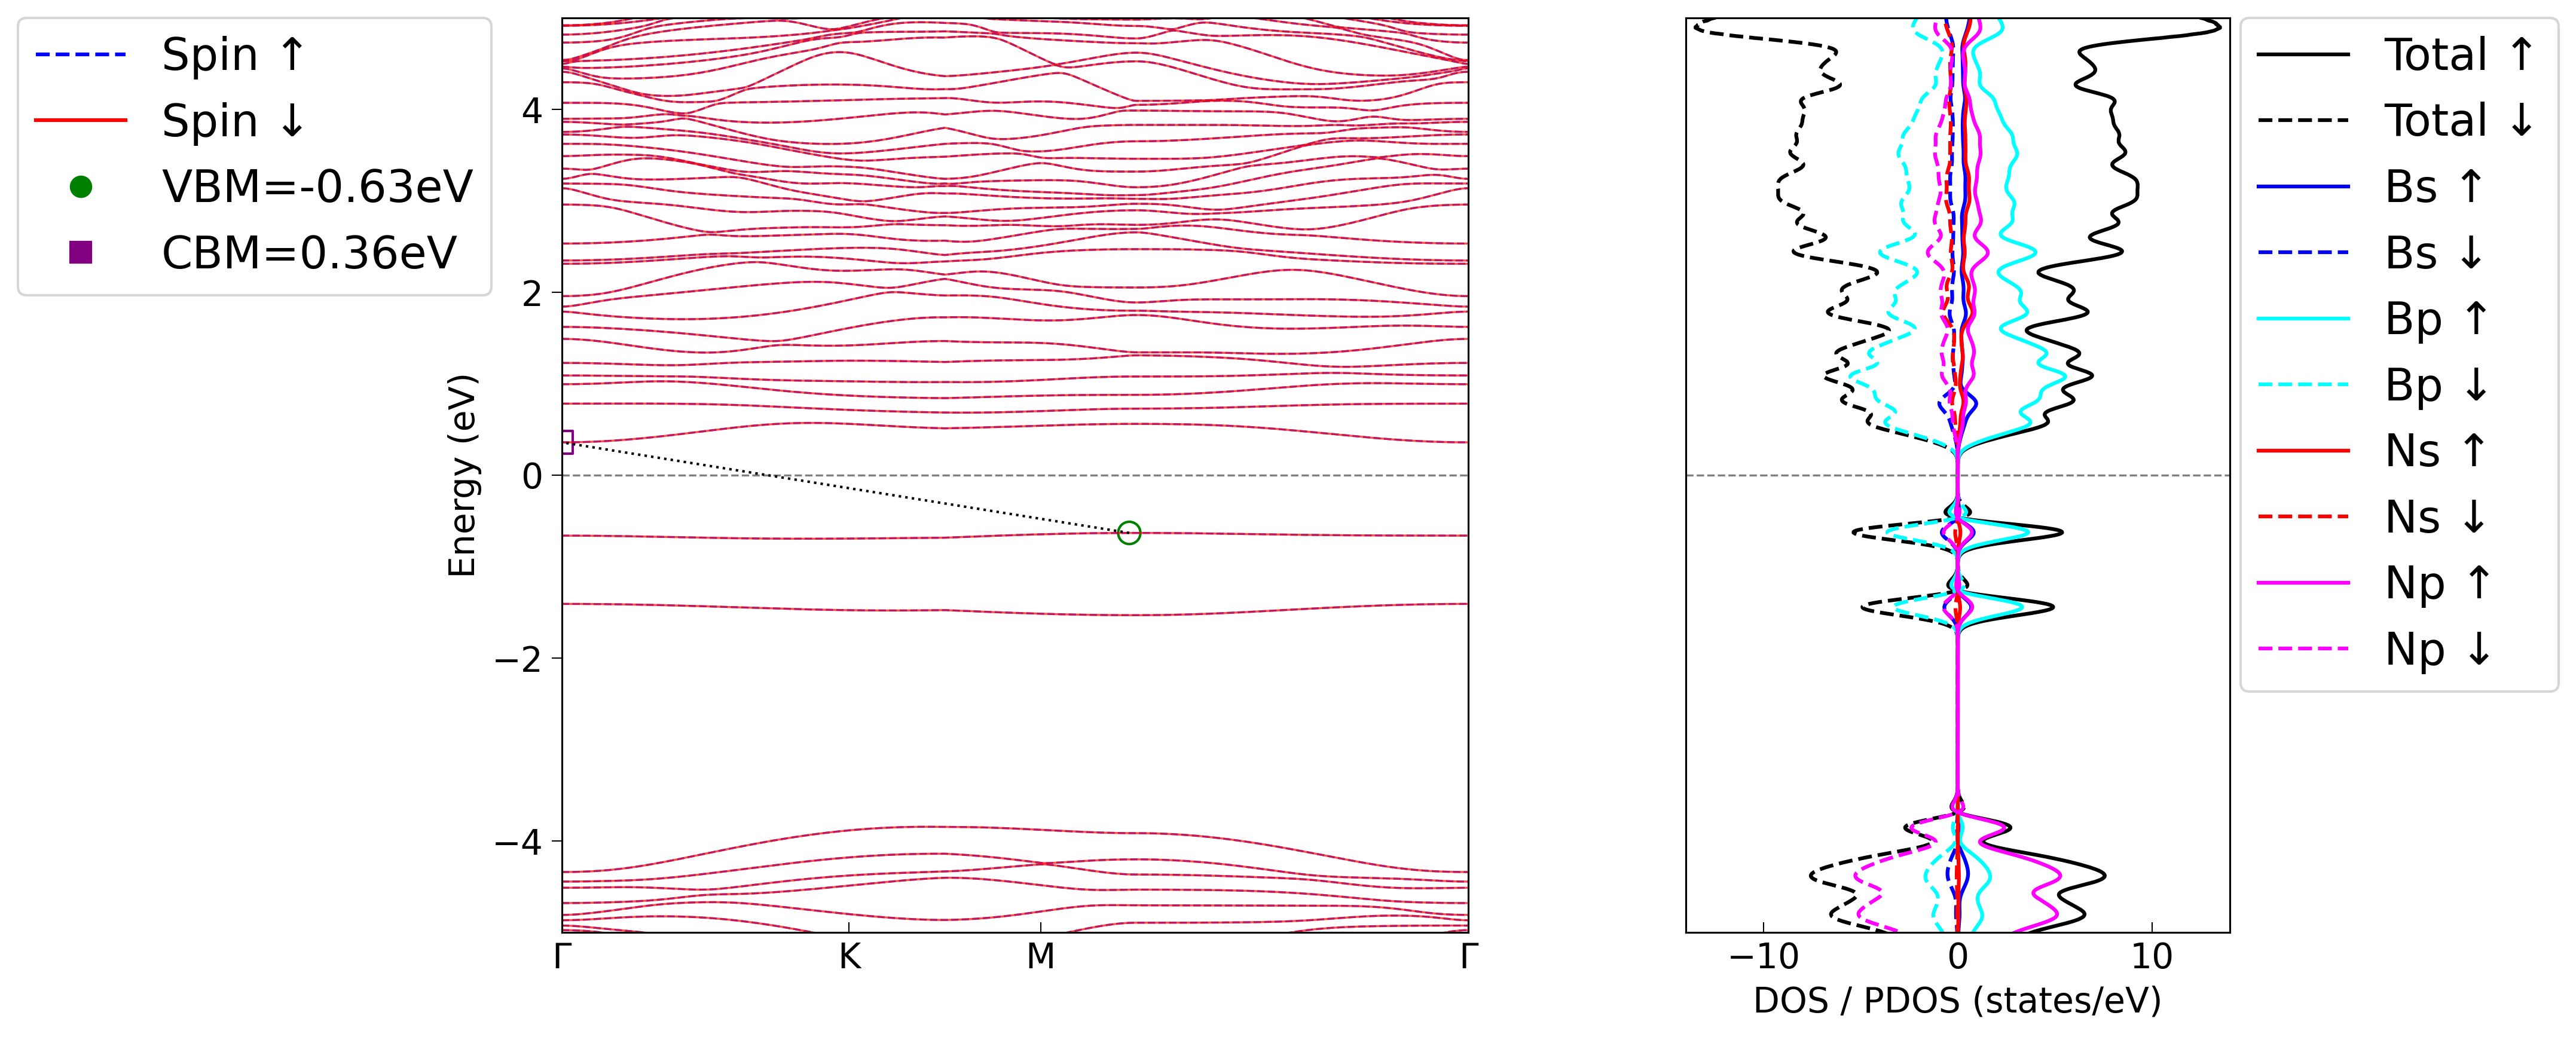
\includegraphics[width=0.9\textwidth]{gambar_hasil/simple_bands_pdos_BB_800K.png}
    \caption{Struktur pita elektronik dan PDOS untuk monolayer hBN dengan defek B$_N$ pada 800K.}
    \label{fig:hbn_BB_800K}
\end{figure}
\begin{figure}[h!]
    \centering
    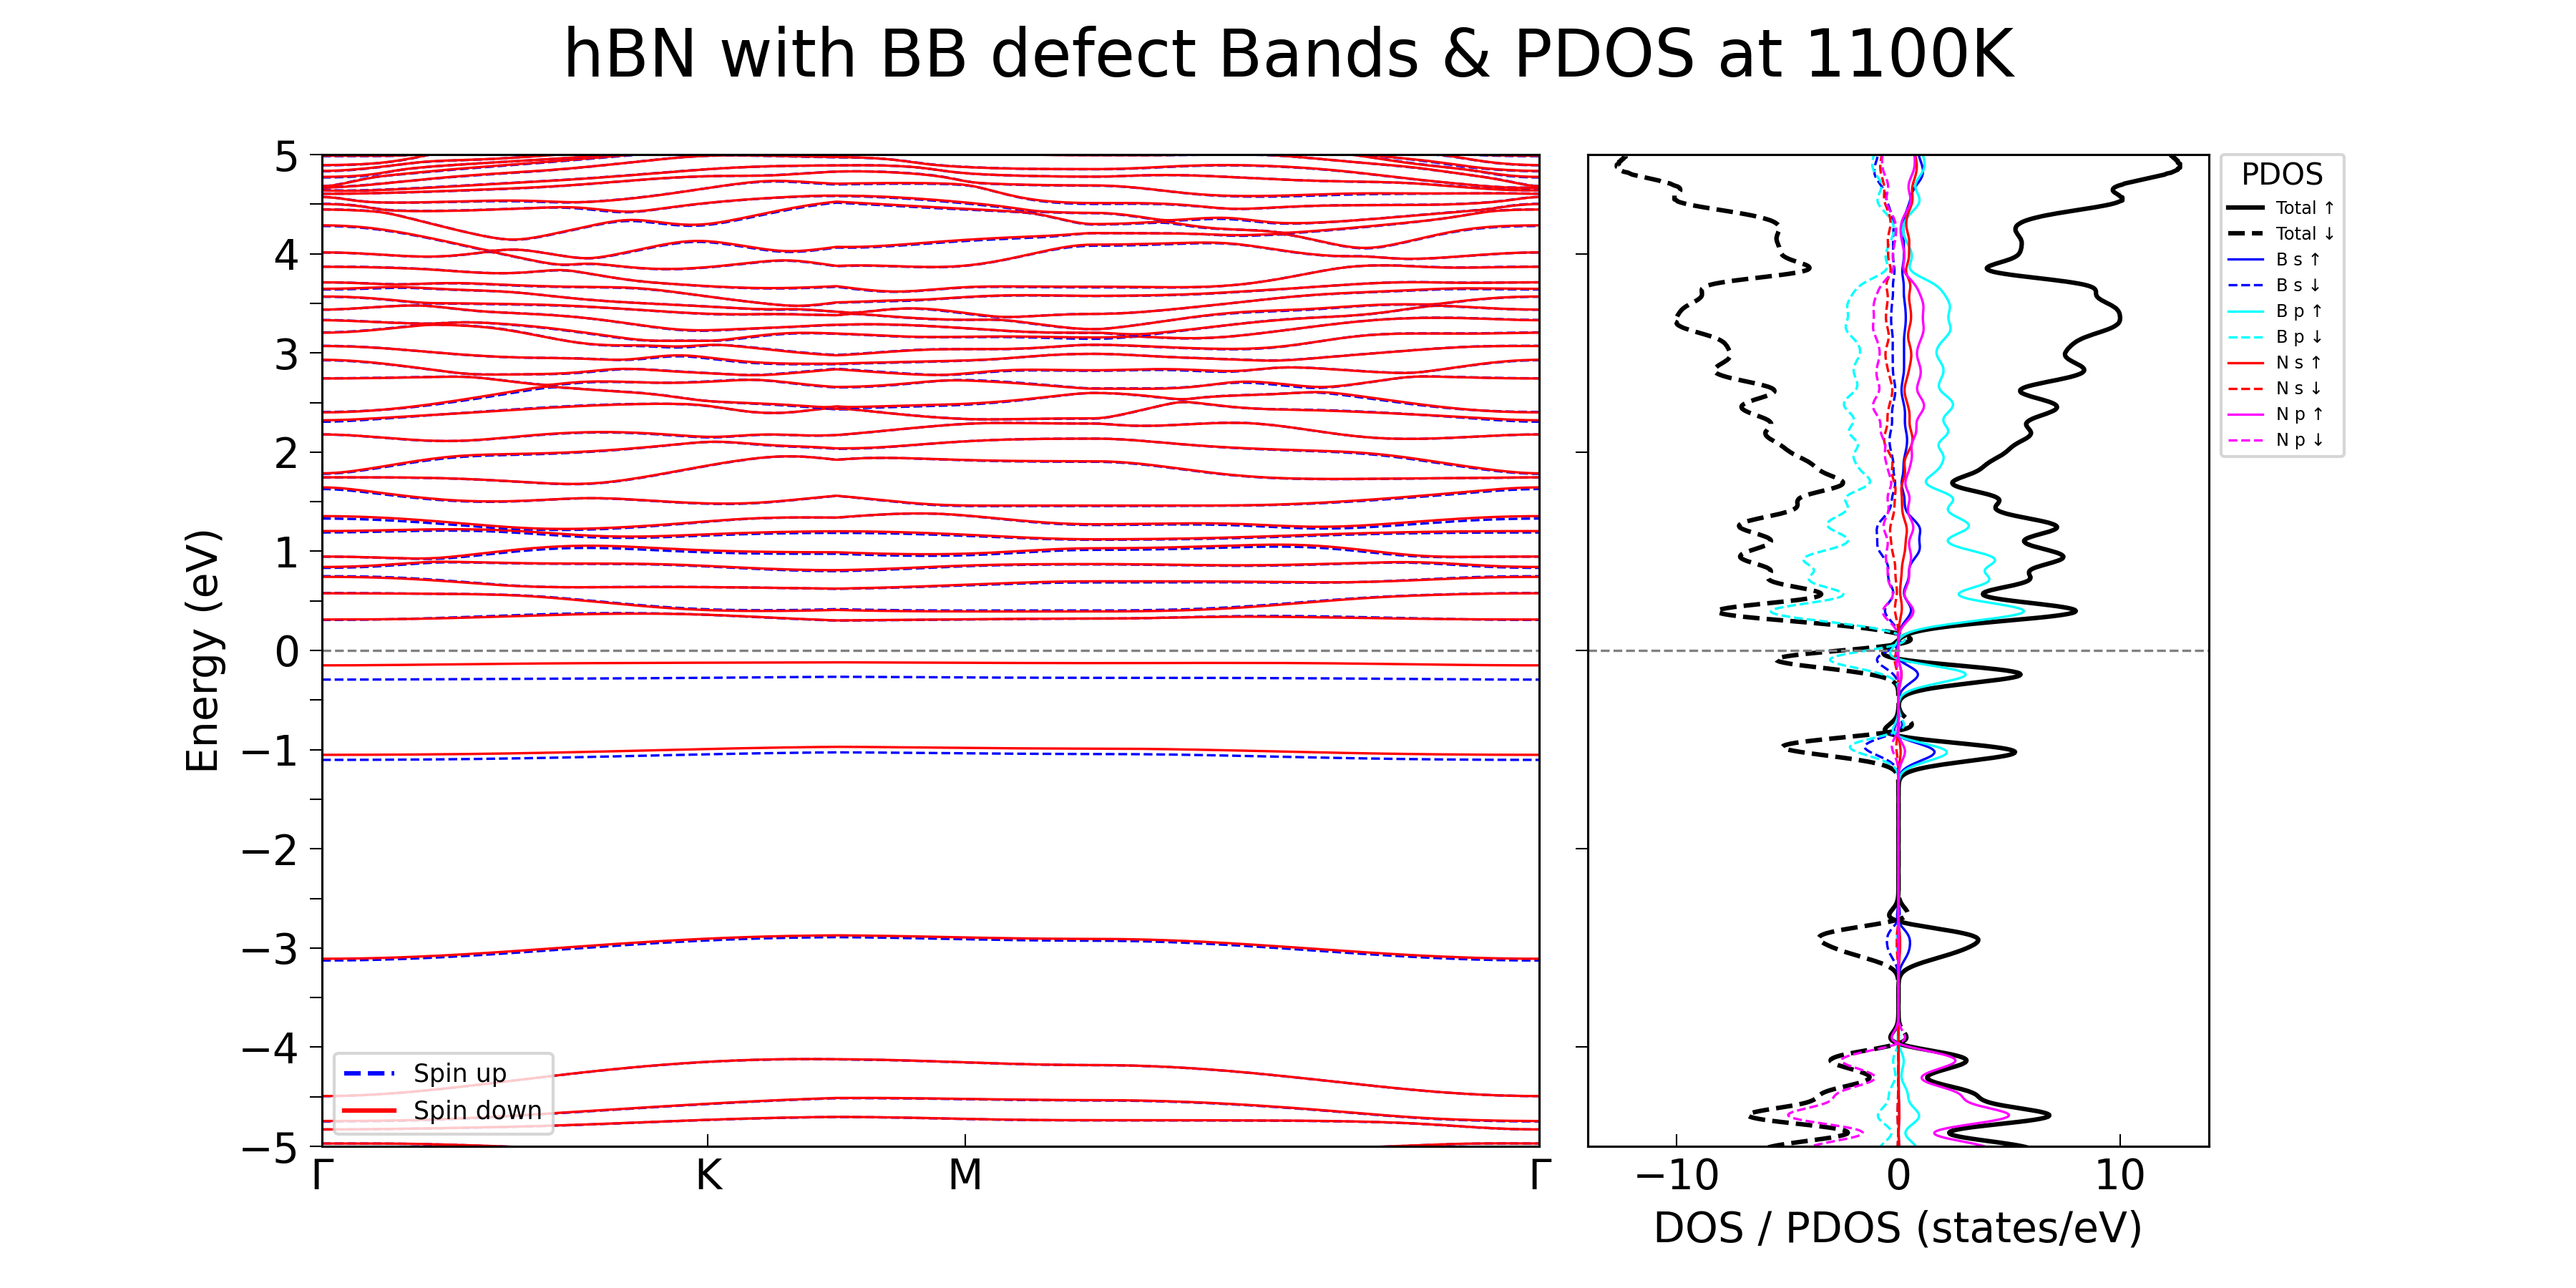
\includegraphics[width=0.9\textwidth]{gambar_hasil/simple_bands_pdos_BB_1100K.png}
    \caption{Struktur pita elektronik dan PDOS untuk monolayer hBN dengan defek B$_N$ pada 1100K, menunjukkan pemisahan spin.}
    \label{fig:hbn_BB_1100K}
\end{figure}
\begin{figure}[h!]
    \centering
    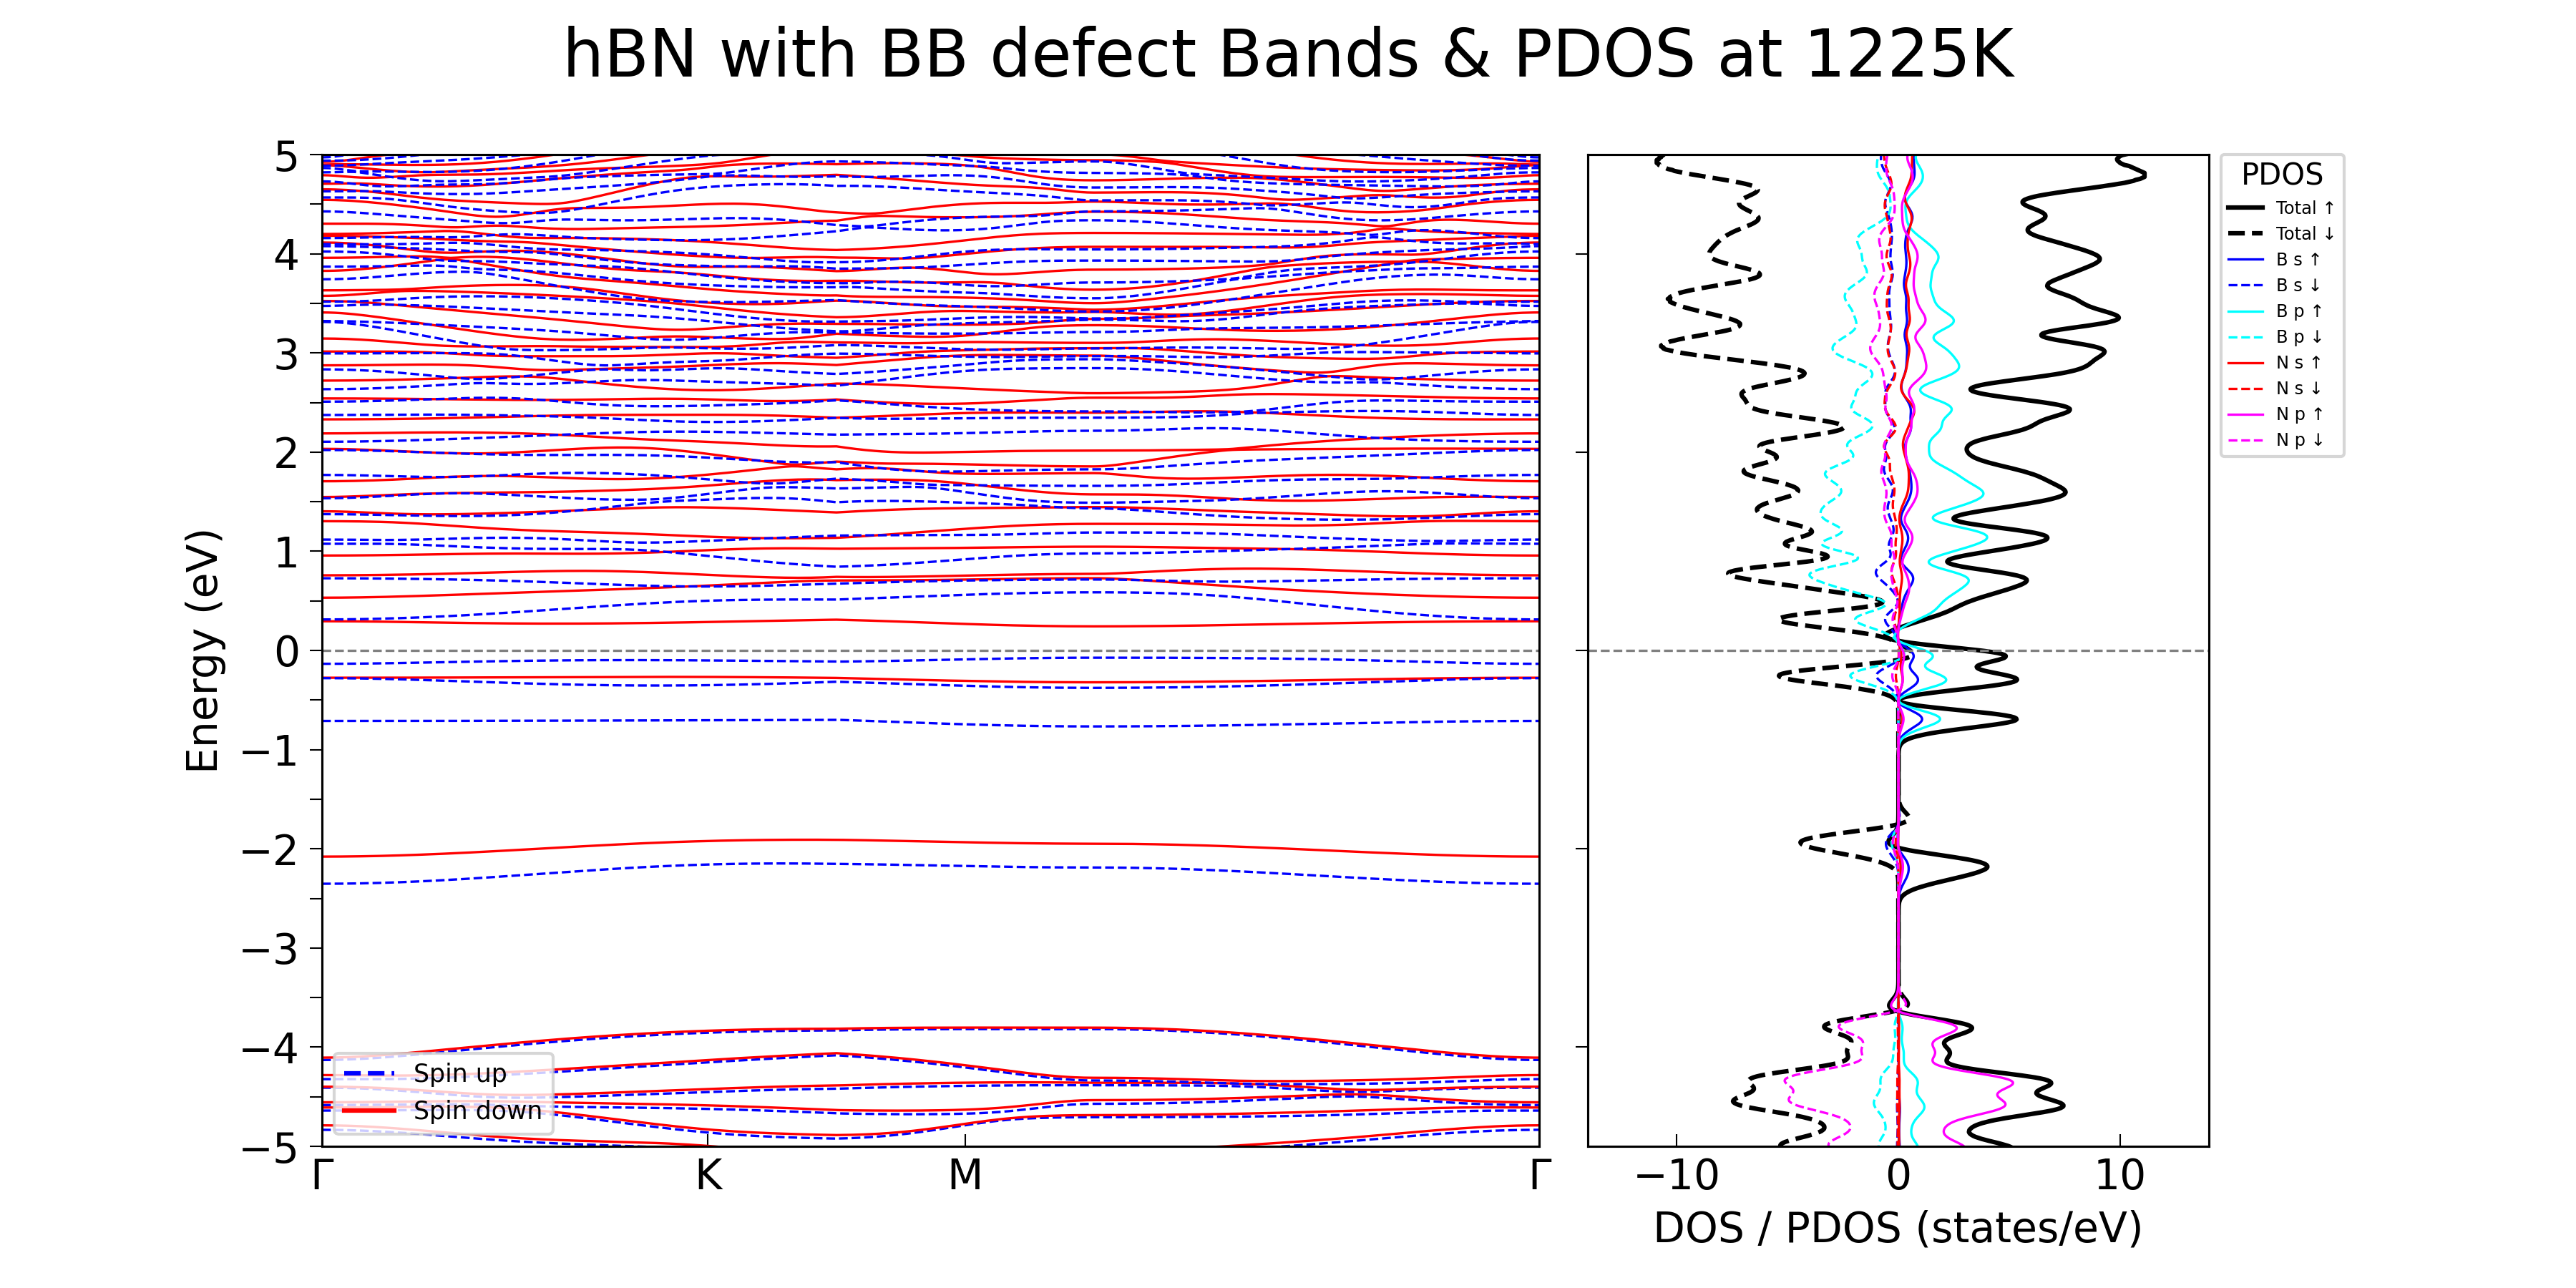
\includegraphics[width=0.9\textwidth]{gambar_hasil/simple_bands_pdos_BB_1225K.png}
    \caption{Struktur pita elektronik dan PDOS untuk monolayer hBN dengan defek B$_N$ pada 1225K, menunjukkan pemisahan spin yang lebih signifikan.}
    \label{fig:hbn_BB_1225K}
\end{figure}
\begin{figure}[h!]
    \centering
    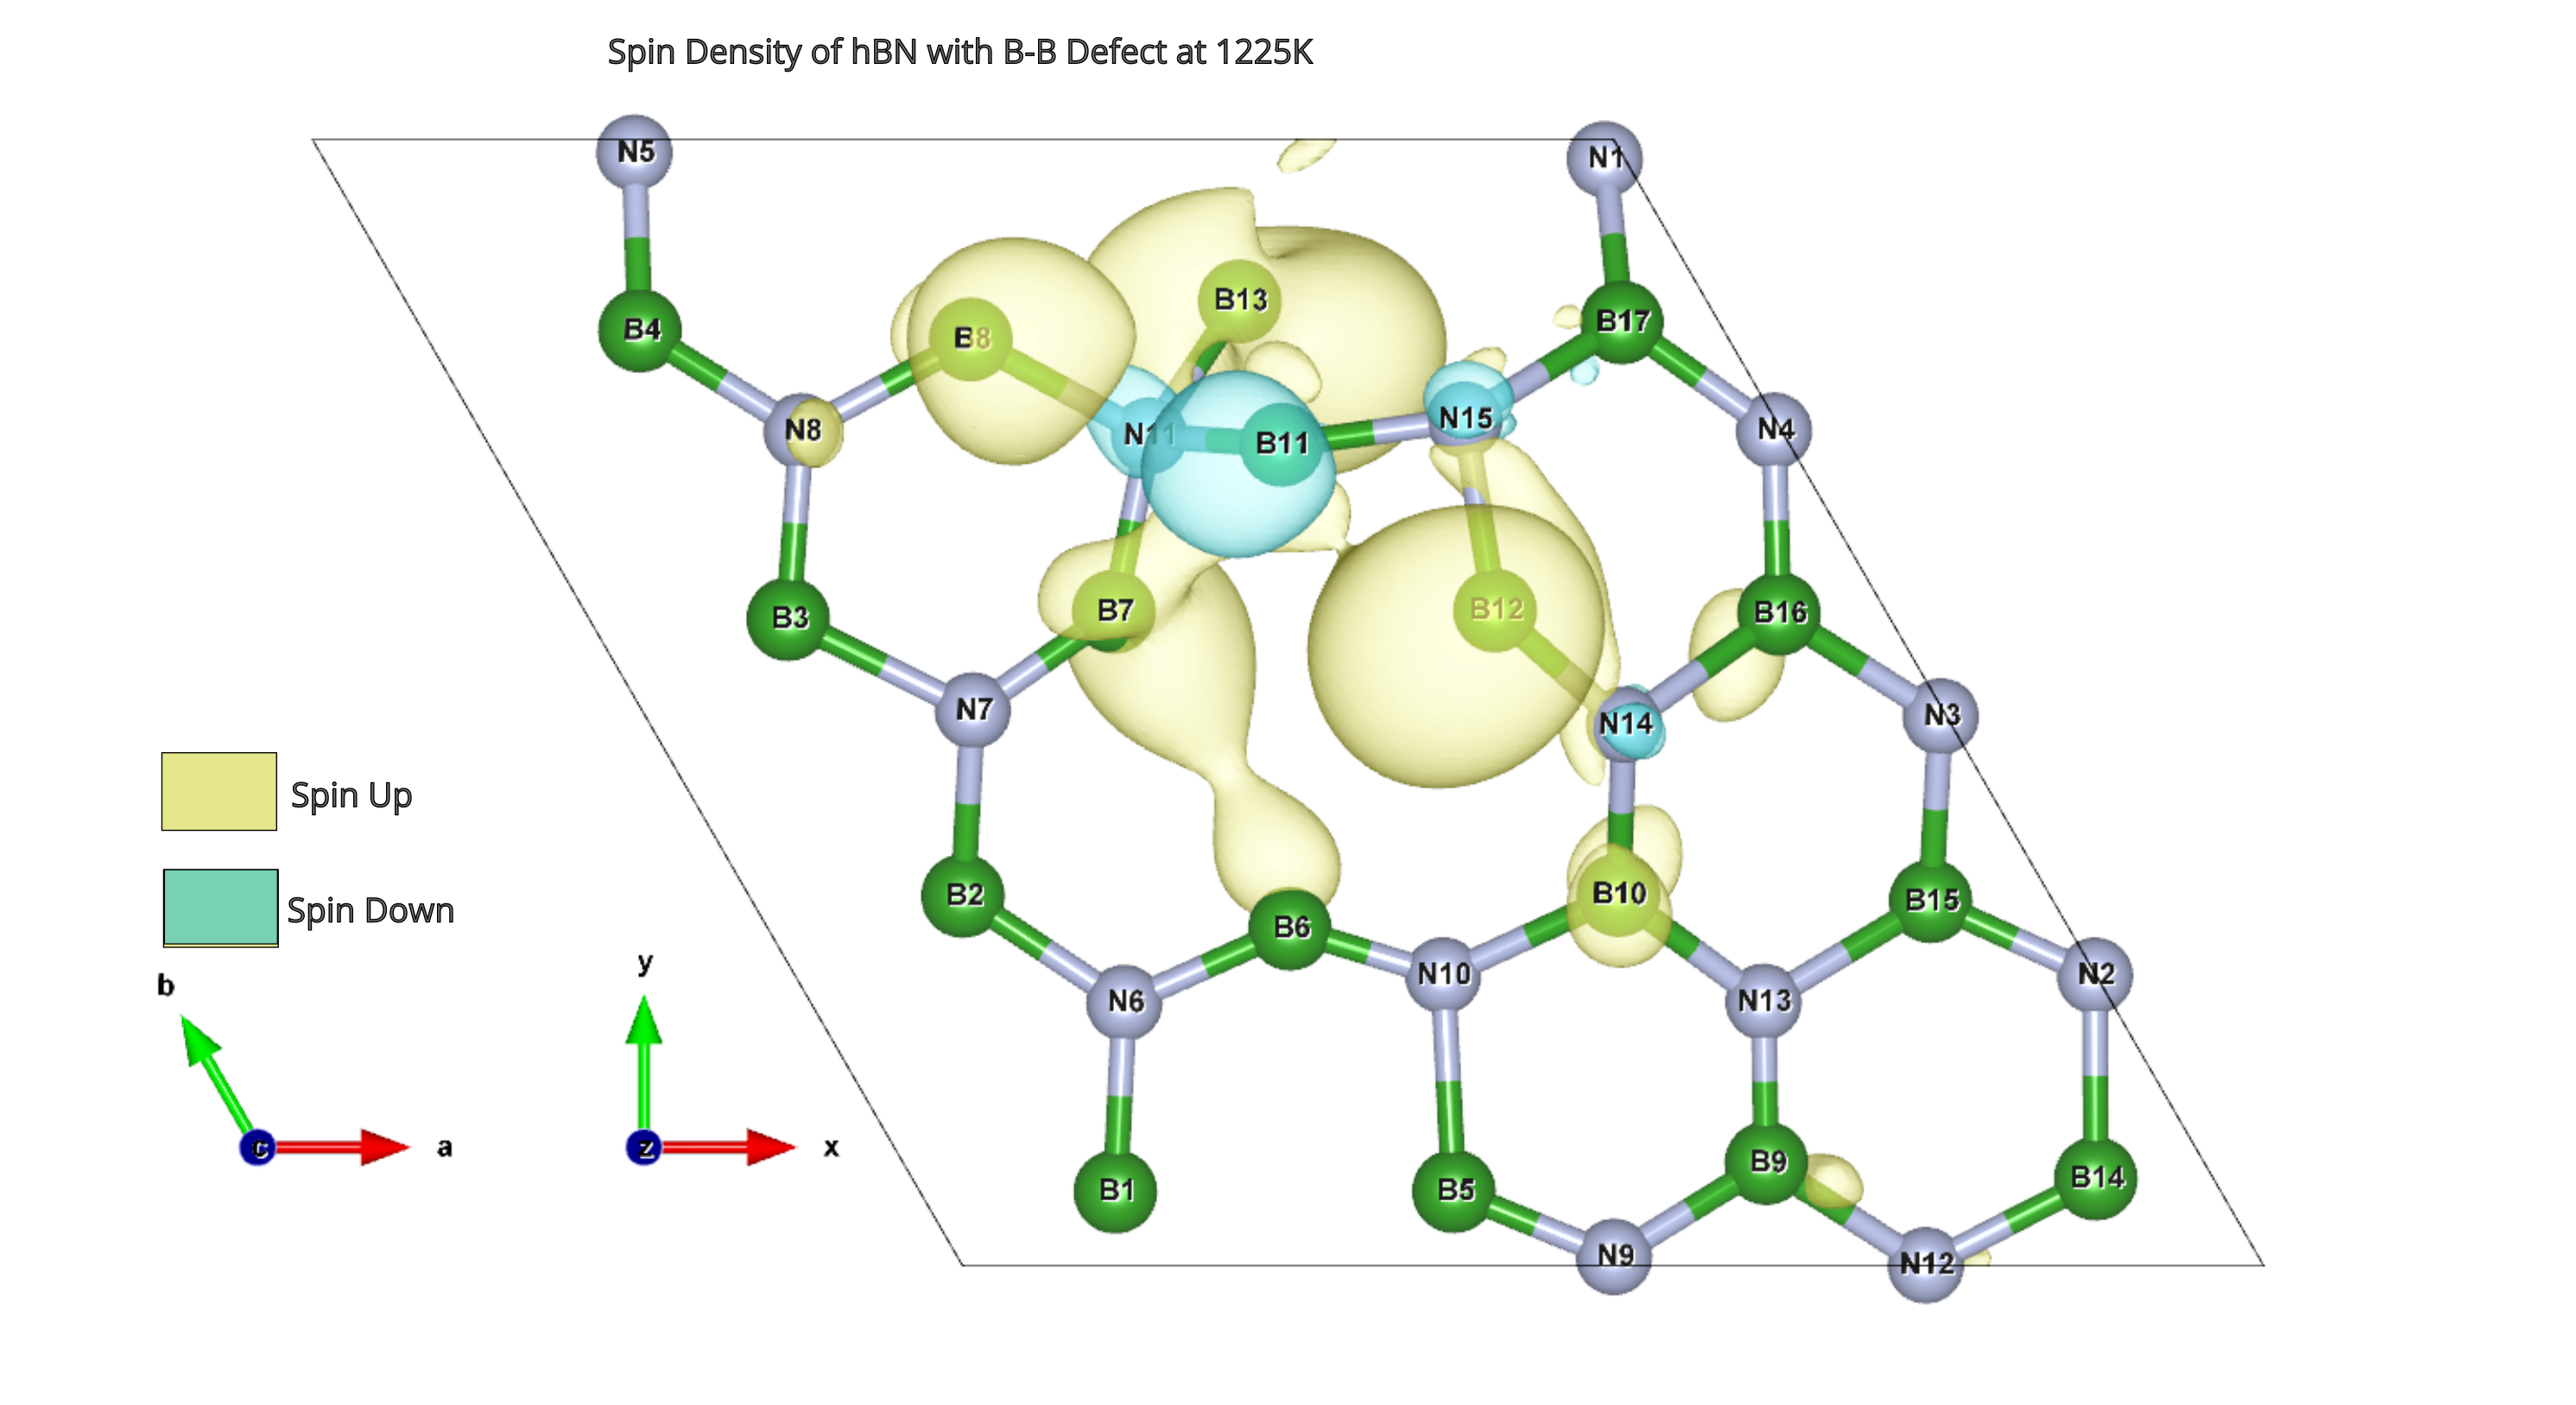
\includegraphics[width=0.6\textwidth]{gambar_hasil/hBN_spin_BB_1225K.png}
    \caption{Visualisasi kerapatan spin 3D untuk monolayer hBN dengan defek B$_N$ pada 1225K, menunjukkan lokalisasi momen magnetik di sekitar situs defek.}
    \label{fig:hbn_BB_1225K_spindensity}
\end{figure}

\subsubsection{Induksi Magnetisme $d^0$ oleh Distorsi Lokal}
Temuan paling signifikan adalah induksi magnetisme yang bergantung pada temperatur. Pada 800K, sistem bersifat non-magnetik. Namun, pada 1100K, momen magnetik total sebesar $0.150 \mu_B$ muncul, dan meningkat tajam menjadi $1.850 \mu_B$ pada 1225K. Kemunculan magnetisme pada sistem yang hanya terdiri dari unsur-unsur blok-p ini dikenal sebagai \textbf{magnetisme $d^0$} \citep{zhou2019}. Magnetisme jenis ini tidak berasal dari orbital $d$ atau $f$ yang terisi sebagian, melainkan dari polarisasi spin elektron-elektron $p$ yang terlokalisasi.

Defek B$_N$ menciptakan kondisi yang ideal untuk ini: sebuah atom Boron (3 elektron valensi) menggantikan Nitrogen (5 elektron valensi) dan dikelilingi oleh tiga atom Boron tetangga. Hal ini menciptakan ketidakseimbangan elektron dan ikatan yang tidak jenuh (\textit{dangling bonds}) yang mengarah pada keadaan elektronik terlokalisasi di dekat tingkat Fermi. Distorsi struktural lokal di sekitar defek, yang ditangkap oleh simulasi MD pada temperatur tinggi, dapat memecah degenerasi orbital (efek mirip Jahn-Teller) dan membuat sistem lebih rentan terhadap polarisasi spin untuk menurunkan energi totalnya, sesuai dengan kriteria Stoner \citep{Zhu2011}. Kerapatan spin yang terlokalisasi di sekitar situs defek, terutama pada atom N tetangga (Gambar \ref{fig:hbn_BB_1225K_spindensity} dan \ref{fig:hbn_BB_1225K_spindensity_2D}), sangat mendukung mekanisme ini.

\subsubsection{Ketergantungan Temperatur Anomali dan Peran Kopling Spin-Fonon}
Peningkatan magnetisasi dengan suhu (dari 800K ke 1225K) adalah fenomena yang sangat tidak biasa dan berlawanan dengan kecenderungan umum di mana energi termal ($k_B T$) mengacaukan tatanan magnetik (menuju temperatur Curie). Perilaku ini menunjukkan adanya mekanisme yang lebih kompleks, kemungkinan besar adalah \textbf{kopling spin-fonon} yang kuat \citep{Liu_2025}.

Hipotesisnya adalah sebagai berikut: pada 800K, distorsi termal pada kisi belum cukup untuk menstabilkan keadaan dasar magnetik. Struktur atomik pada temperatur ini, ketika dihitung dengan DFT, menghasilkan keadaan dasar non-magnetik. Seiring dengan meningkatnya temperatur ke 1100K dan 1225K, mode-mode fonon dengan amplitudo yang lebih besar menjadi aktif. Jika mode-mode fonon spesifik ini berinteraksi kuat dengan keadaan elektronik di sekitar defek B$_N$, mereka dapat secara dinamis mempertahankan atau bahkan memperkuat distorsi lokal yang kondusif untuk polarisasi spin. Dengan kata lain, vibrasi kisi pada suhu tinggi tidak hanya bertindak sebagai sumber kekacauan, tetapi juga secara aktif menstabilkan konfigurasi atomik yang bersifat magnetik. Sistem pada 800K mungkin berada di dekat titik transisi fasa magnetik, dan temperatur yang lebih tinggi mendorongnya lebih dalam ke fase magnetik yang lebih teratur. Fenomena di mana getaran kolektif dapat memediasi atau menstabilkan tatanan jarak jauh merupakan area penelitian yang sangat aktif, dengan beberapa teori baru yang mengeksplorasi bagaimana kopling dengan fonon atau bahkan foton dapat mengarah pada magnetisme yang tidak konvensional \citep{Pantazopoulos2024}.

Sekali lagi, validitas temuan yang luar biasa ini sangat bergantung pada keakuratan struktur yang dihasilkan oleh potensial ReaxFF pada temperatur tinggi. Jika potensial tersebut melebih-lebihkan distorsi lokal tertentu sebagai respons terhadap suhu, maka magnetisme yang dihasilkan bisa jadi merupakan artefak.

\section{Diskusi Komprehensif dan Implikasi Hasil}
\label{sec:diskusi_komprehensif}
Analisis terhadap monolayer hBN murni dan yang mengandung defek antisite N$_B$ serta B$_N$ pada berbagai temperatur mengungkapkan perilaku material yang kompleks dan menarik, dengan implikasi signifikan bagi rekayasa material dan aplikasi perangkat.

\subsection{Analisis Perbandingan Celah Pita Energi Antar Sistem}
\label{subsec:perbandingan_eg}
Perbandingan sistematis tren celah pita energi ($E_g$) sebagai fungsi temperatur (T) menunjukkan perilaku yang sangat beragam (dirangkum dalam Tabel \ref{tab:konsolidasi_eg_mag}):
\begin{itemize}
    \item \textbf{hBN Murni:} Menunjukkan redshift normal ($E_g$ menurun dengan T), yang kemungkinan besar merupakan cerminan dari dominasi kopling elektron-fonon pada rentang temperatur tinggi, dengan potensi artefak dari ketiadaan efek NTE dalam model.
    \item \textbf{hBN + Defek N$_B$:} Menunjukkan blueshift anomali ($E_g$ meningkat dengan T). Ini mengindikasikan bahwa kopling elektron-fonon yang terlokalisasi pada defek ini memiliki sifat yang berbeda secara kualitatif, di mana vibrasi termal justru meningkatkan pemisahan energi antara keadaan defek.
    \item \textbf{hBN + Defek B$_N$:} Menunjukkan redshift normal, mirip dengan hBN murni, meskipun dengan nilai $E_g$ yang jauh lebih kecil. Ini menyiratkan bahwa mekanisme yang mengatur $E_g(T)$ pada sistem ini lebih mirip dengan material induknya.
\end{itemize}
Keragaman perilaku $E_g(T)$ ini menunjukkan bahwa rekayasa defek tidak hanya memodifikasi nilai $E_g$ absolut tetapi juga dapat mengubah koefisien temperatur dari $E_g$, sebuah properti penting untuk stabilitas termal perangkat optoelektronik.

\subsection{Asal Usul dan Sifat Magnetisme pada hBN dengan Defek B$_N$}
\label{subsec:asal_magnetisme_bn}
Temuan paling menonjol adalah induksi magnetisme $d^0$ oleh defek B$_N$ yang meningkat dengan temperatur. Fenomena ini, jika terbukti nyata dan bukan artefak metodologi, merupakan contoh menarik dari magnetisme yang diinduksi oleh defek. Ketergantungan temperatur yang anomali menunjuk pada peran penting kopling spin-fonon, di mana vibrasi kisi pada suhu tinggi secara aktif menstabilkan keadaan magnetik. Perlu ditekankan kembali bahwa temuan ini sangat sensitif terhadap akurasi struktur atomik yang dihasilkan oleh simulasi MD, dan memerlukan validasi lebih lanjut dengan potensial interatomik yang lebih akurat seperti MLIPs.

\subsection{Interplay Kritis antara Dinamika Struktural MD dan Sifat Kuantum DFT}
\label{subsec:korelasi_struktur_md_dft}
Seluruh kalkulasi DFT dalam penelitian ini didasarkan pada struktur atomik dari simulasi MD. Alur kerja multi-skala ini menggarisbawahi sebuah poin krusial: DFT secara akurat menghitung sifat elektronik untuk konfigurasi atomik yang *diberikan*, namun jika struktur input itu sendiri tidak merepresentasikan realitas fisik, maka sifat akhir yang diprediksi bisa jadi bias atau bahkan salah secara kualitatif.

Fenomena-fenomena paling signifikan yang teramati dalam studi ini—(1) tren redshift $E_g(T)$ pada hBN murni yang kontras dengan ekspektasi blueshift, (2) tren blueshift $E_g(T)$ anomali untuk defek N$_B$, dan (3) magnetisme yang meningkat dengan temperatur untuk defek B$_N$—kemungkinan besar sangat dipengaruhi oleh konfigurasi atomik spesifik yang dihasilkan MD pada setiap temperatur. Keandalan struktur-struktur ini, mengingat potensial ReaxFF yang digunakan \citep{Lele2022} diparameterisasi untuk sintesis fasa gas, menjadi pertanyaan sentral. Masalahnya bergeser dari "apakah DFT memprediksi magnetisme untuk struktur ini?" menjadi "apakah struktur ini secara fisik realistis?".

Studi ini secara efektif menjadi studi kasus tentang pentingnya validasi silang dalam pemodelan multi-skala. Hasil yang paling menarik harus dipandang bukan sebagai prediksi definitif, melainkan sebagai hipotesis yang menarik, yang validitasnya bergantung sepenuhnya pada keakuratan potensial MD yang digunakan untuk menangkap fisika fasa padat yang relevan.

\subsection{Implikasi Temuan untuk Aplikasi Potensial}
\label{subsec:implikasi_aplikasi}
Meskipun memerlukan validasi lebih lanjut, temuan dari penelitian ini memiliki beberapa implikasi penting untuk potensi aplikasi monolayer hBN:
\begin{itemize}
    \item \textbf{Optoelektronika:} Kemampuan menyetel celah pita dari UV-dalam hingga rentang tampak/inframerah-dekat melalui rekayasa defek membuka peluang untuk fotodetektor dan emitor cahaya yang dapat diatur. Ketergantungan temperatur yang berbeda dari $E_g$ untuk defek N$_B$ dan B$_N$ perlu dipertimbangkan dalam desain perangkat.
    \item \textbf{Spintronika:} Induksi sifat magnetik oleh defek B$_N$ menunjukkan potensi penggunaan hBN dalam komponen spintronik seperti filter spin atau memori magnetik berbasis material 2D. Ketergantungan temperatur yang anomali, jika nyata, dapat dieksploitasi untuk sensor termal-spin atau sakelar magnetik yang diaktifkan oleh panas.
    \item \textbf{Sensor:} Perubahan sifat elektronik yang sensitif terhadap jenis defek dan temperatur dapat dieksploitasi untuk pengembangan sensor kimia atau temperatur presisi.
\end{itemize}
Secara keseluruhan, penelitian ini menunjukkan bahwa monolayer hBN bukan hanya isolator pasif, tetapi material yang sifat-sifatnya dapat dimodulasi secara aktif melalui kontrol kondisi termal dan rekayasa defek, membuka jalan bagi fungsionalitas baru.

\begin{table}[h!]
  \centering
  \caption{Tinjauan Konsolidasi Celah Pita Energi dan Magnetisasi Total untuk Semua Sistem yang Dikaji.}
  \label{tab:konsolidasi_eg_mag}
  \begin{tabular}{llcc}
    \toprule
    Sistem & Temperatur (K) & Celah Pita Energi ($E_g$) (eV) & Magnetisasi Total ($\mu_B$) \\
    \midrule
    hBN Murni & Pristine & 4.446 & 0.000 \\
              & 800      & 4.415 & 0.000 \\
              & 1100     & 4.328 & 0.000 \\
              & 1225     & 4.069 & 0.000 \\
    \midrule
    hBN + Defek N$_B$ & 800  & 0.694 &  0.000 \\
                      & 1100 & 1.089 &  0.000 \\
                      & 1225 & 1.214 &  0.000 \\
    \midrule
    hBN + Defek B$_N$ & 800  & 0.990 &  0.000 \\
                      & 1100 & 0.421 &  0.150 \\
                      & 1225 & 0.316 &  1.850 \\
    \bottomrule
  \end{tabular}
\end{table}